\chapter{Hiện thực hệ thống}
\label{chap:3}


Chương này trình bày cách nhóm hiện thực Nene dựa trên thiết kế ở Chương~\ref{chap:2}: môi trường và công cụ phát triển, cấu trúc mã nguồn, cách hiện thực từng nhóm chức năng của đề bài, cơ sở dữ liệu (CSDL) và bảo mật dữ liệu, cách triển khai và cách tổ chức kiểm thử tự động. Mọi mô tả bám theo mã nguồn trên nhánh \texttt{main} tại commit \texttt{bfdab0c}. Các đoạn mã được trích từ mã nguồn thật; một số đoạn được rút gọn hoặc gộp dòng cho vừa trang, phần lược bỏ được đánh dấu bằng chú thích \texttt{/\allowbreak{}/ ...} hoặc \texttt{-- ...}. Giao diện ứng dụng hiện dùng tiếng Anh, vì vậy tên màn hình và nút bấm được giữ nguyên khi nhắc đến.

Trong chương này, ``dữ liệu tổng hợp'' (synthetic data) là dữ liệu do nhóm tự tạo cho mục đích demo; ``giả lập'' (simulated) là chức năng mô phỏng một dịch vụ thật nhưng không kết nối dịch vụ thật; ``sandbox'' là môi trường thử nghiệm do nhà cung cấp (ở đây là VNPay) cung cấp, không phát sinh giao dịch tiền thật.

%=====================================================================
\section{Môi trường và công cụ phát triển}
\label{sec:ch3-env}

Nene gồm ba phần chạy độc lập: (1) ứng dụng Android viết bằng Flutter/Dart; (2) một giao diện lập trình ứng dụng (API) duy nhất viết bằng NestJS/TypeScript, chạy trên Node.js; (3) Supabase, cung cấp PostgreSQL, dịch vụ xác thực (Auth) và kho tệp riêng tư (Storage). Khi phát triển cục bộ, Supabase CLI chạy toàn bộ các dịch vụ Supabase trong Docker trên máy của nhóm, nên mọi chức năng có thể chạy thử mà không cần tài khoản đám mây. Bảng~\ref{tab:ch3-tools} liệt kê các công cụ chính và phiên bản đã dùng để kiểm tra.

\begin{table}[H]
	\centering
	\caption{Công cụ và môi trường phát triển}
	\label{tab:ch3-tools}
	\small
	\begin{tabularx}{\textwidth}{@{}>{\raggedright\arraybackslash}p{4.2cm}>{\raggedright\arraybackslash}p{2.6cm}X@{}}
		\toprule
		\textbf{Công cụ} & \textbf{Phiên bản} & \textbf{Vai trò trong dự án}\\
		\midrule
		Flutter (kênh stable), Dart & 3.47.7; 3.13.5 & Xây dựng ứng dụng Android. Bản web debug của cùng mã nguồn chỉ dùng để xem trước cục bộ trên trình duyệt, không phải sản phẩm phát hành \parencite{ch3-flutter-docs}.\\
		Android SDK, JDK 17, Gradle (Kotlin DSL) & theo Flutter & Biên dịch và ký gói phát hành Android App Bundle (AAB).\\
		Node.js, npm & 24; 11 & Môi trường chạy API và các script kiểm tra.\\
		NestJS, TypeScript & 12.1.3; 6.0.3 & Framework API; mã được biên dịch trực tiếp bằng \texttt{tsc}, không cần Nest CLI \parencite{ch3-nestjs-docs}.\\
		PostgreSQL (do Supabase cung cấp) & dịch vụ Supabase & CSDL quan hệ duy nhất của ứng dụng.\\
		Supabase CLI, Docker Desktop & 2.121.0 & Chạy Supabase cục bộ, áp dụng migration và đẩy migration lên Supabase cloud \parencite{ch3-supabase-migrations}.\\
		Git, GitHub & -- & Quản lý mã nguồn. Mỗi thay đổi được thực hiện trên một nhánh riêng và gộp vào \texttt{main} qua pull request.\\
		Visual Studio Code & -- & Trình soạn thảo chính; ESLint, Prettier và \texttt{flutter analyze} dùng để kiểm tra mã.\\
		\bottomrule
	\end{tabularx}
\end{table}

Dự án chưa cấu hình hệ thống tích hợp liên tục (CI). Trước khi mở pull request, nhóm chạy các lệnh kiểm tra cục bộ được ghi trong tài liệu \texttt{docs/\allowbreak{}SETUP.\allowbreak{}md}: \texttt{npm --prefix backend run check} (lint, biên dịch và kiểm thử backend), \texttt{flutter analyze} và \texttt{flutter test} (trong thư mục \texttt{app/}). Bảng~\ref{tab:ch3-libs} tóm tắt các thư viện chính và mục đích sử dụng; phiên bản được khóa cố định trong \texttt{pubspec.\allowbreak{}yaml}, \texttt{pubspec.\allowbreak{}lock}, \texttt{package.\allowbreak{}json} và \texttt{package-\allowbreak{}lock.\allowbreak{}json}.

\begin{table}[H]
	\centering
	\caption{Thư viện chính và mục đích sử dụng}
	\label{tab:ch3-libs}
	\footnotesize
	\begin{tabularx}{\textwidth}{@{}>{\raggedright\arraybackslash}p{5.6cm}X@{}}
		\toprule
		\textbf{Thư viện (phiên bản)} & \textbf{Mục đích}\\
		\midrule
		\multicolumn{2}{@{}l}{\textit{Ứng dụng Flutter (\texttt{app/\allowbreak{}pubspec.\allowbreak{}yaml})}}\\
		\texttt{http} 1.6.0 & Gọi REST API của backend và các endpoint của Supabase Auth.\\
		\texttt{flutter\_\allowbreak{}map} 8.3.2, \texttt{latlong2} 0.9.1 & Hiển thị bản đồ ô gạch OpenStreetMap, vị trí người dùng, văn phòng và tuyến đường \parencite{ch3-flutter-map}.\\
		\texttt{geolocator} 14.1.2 & Kiểm tra, xin quyền vị trí và đọc vị trí hiện tại \parencite{ch3-geolocator}.\\
		\texttt{image\_\allowbreak{}picker} 1.2.4 & Chụp ảnh tham chiếu bằng camera trước.\\
		\texttt{google\_mlkit\_\allowbreak face\_detection} 1.0.3 & Phát hiện khuôn mặt ngay trên thiết bị Android; mô hình được đóng gói sẵn trong ứng dụng \parencite{ch2-mlkit-face}.\\
		\texttt{url\_\allowbreak{}launcher} 6.3.3 & Mở trang thanh toán VNPay sandbox và các liên kết bản quyền bản đồ bằng ứng dụng bên ngoài.\\
		\texttt{supabase\_\allowbreak{}flutter} 2.18.3 & SDK của Supabase. Hiện chỉ được một adapter cũ dùng trong bộ kiểm thử hồi quy; luồng đăng nhập chính dùng adapter do nhóm tự viết (Mục~\ref{sec:ch3-auth}).\\
		\texttt{flutter\_\allowbreak{}test}, \texttt{flutter\_\allowbreak{}lints} & Kiểm thử widget/unit và luật phân tích tĩnh.\\
		Phông Be Vietnam Pro (SIL OFL 1.1) & Đóng gói trong ứng dụng để hiển thị đúng dấu tiếng Việt mà không phải tải phông qua mạng.\\
		\midrule
		\multicolumn{2}{@{}l}{\textit{Backend NestJS (\texttt{backend/\allowbreak{}package.\allowbreak{}json})}}\\
		\texttt{@nestjs/\allowbreak{}common}, \texttt{@nestjs/\allowbreak{}core}, \texttt{@nestjs/\allowbreak{}platform-\allowbreak{}express} 12.1.3; \texttt{express} 5.2.1 & Framework HTTP, cơ chế tiêm phụ thuộc (dependency injection) và guard toàn cục \parencite{ch2-nestjs-guards}.\\
		\texttt{pg} 8.23.1 & Driver PostgreSQL. Mọi truy vấn được viết bằng SQL tham số hóa (\texttt{\$1}, \texttt{\$2}, \ldots), không dùng ORM \parencite{ch3-node-postgres}.\\
		\texttt{@supabase/\allowbreak{}supabase-\allowbreak{}js} 2.117.3 & Xác minh phiên với Supabase Auth, tạo tài khoản đăng nhập qua Admin API, đọc/ghi Storage riêng tư.\\
		\texttt{sharp} 0.35.5 & Giải mã, xoay đúng chiều và mã hóa lại ảnh tham chiếu \parencite{ch3-sharp}.\\
		\texttt{dotenv} 18.0.8 & Nạp biến môi trường cục bộ từ tệp \texttt{.\allowbreak{}env} (tệp này không được đưa vào Git).\\
		\texttt{eslint}, \texttt{typescript-\allowbreak{}eslint}, \texttt{prettier} & Kiểm tra và định dạng mã TypeScript.\\
		\texttt{@nestjs/\allowbreak{}testing}, \texttt{supertest} & Dựng module NestJS và gửi yêu cầu HTTP trong kiểm thử.\\
		\bottomrule
	\end{tabularx}
\end{table}

Hai quyết định ảnh hưởng trực tiếp đến cách viết mã. Thứ nhất, ứng dụng Flutter không dùng thư viện quản lý trạng thái bên ngoài mà dùng lớp \texttt{Change\allowbreak{}Notifier} có sẵn của Flutter. Thứ hai, backend không dùng ORM: SQL tham số hóa giúp nhóm kiểm soát rõ giao dịch CSDL, khóa dòng (\texttt{FOR UPDATE}) và thứ tự khóa trong các thao tác tài chính, đồng thời vẫn tránh được lỗi chèn mã SQL (SQL injection).

%=====================================================================
\section{Cấu trúc mã nguồn}
\label{sec:ch3-structure}

\subsection{Tổ chức kho mã}
\label{sec:ch3-repo}

Toàn bộ dự án nằm trong một kho Git duy nhất. Đoạn mã~\ref{lst:ch3-tree} thể hiện các thư mục chính.

\begin{lstlisting}[caption={Cấu trúc thư mục chính của kho mã Nene},label={lst:ch3-tree}]
nene/
|-- app/                      # Flutter application (package nene_app)
|   |-- lib/
|   |   |-- main.dart         # composition root
|   |   |-- nene_app.dart     # root widget, sign-in, role routing
|   |   |-- session_controller.dart
|   |   |-- customer_flow_controller.dart
|   |   |-- identity_controller.dart
|   |   |-- assistant_controller.dart
|   |   |-- config/           # app_config.dart
|   |   |-- data/             # API clients, repositories, device adapters
|   |   `-- ui/               # screens, nene_brand.dart, nene_components.dart
|   |-- android/              # Gradle project, release signing
|   |-- assets/fonts/         # Be Vietnam Pro
|   |-- config/               # *.example.json for --dart-define-from-file
|   `-- test/                 # widget/unit tests, gated UI capture tests
|-- backend/                  # NestJS API (nene-api)
|   |-- src/
|   |   |-- main.ts, configure-app.ts, app.module.ts
|   |   |-- auth/  profiles/  customers/  identity/  security/
|   |   |-- confirmation/  accounts/  payments/  branches/  assistant/
|   |   `-- config/  database/  health/
|   |-- certs/                # public Supabase root CA certificate
|   `-- test/                 # node:test unit and HTTP specs
|-- infrastructure/
|   `-- supabase/
|       |-- config.toml       # local Supabase settings
|       |-- migrations/       # 17 SQL migrations
|       `-- tests/database/   # pgTAP tests
|-- scripts/                  # seed, migration and integration checks
|-- docs/                     # feature, setup, API and release documents
|-- experiments/              # isolated prototypes, not used by the app
`-- package.json              # workspace commands (db:*, check:*)
\end{lstlisting}

Thư mục \texttt{app/} chứa ứng dụng di động; \texttt{backend/} chứa API; \texttt{infrastructure/\allowbreak{}supabase/} chứa cấu hình Supabase cục bộ, các migration SQL và bộ kiểm thử CSDL; \texttt{scripts/} chứa các script Node.js để chuẩn bị dữ liệu demo và chạy kiểm tra tích hợp; \texttt{docs/} ghi lại quy tắc nghiệp vụ, giới hạn và bằng chứng kiểm tra của từng chức năng. Thư mục \texttt{experiments/} và thư mục \texttt{backend/\allowbreak{}src/\allowbreak{}authorization-\allowbreak{}prototype/} chứa các nguyên mẫu thử nghiệm độc lập về phiên và ủy quyền; chúng không được đăng ký trong ứng dụng đang chạy.

\subsection{Backend NestJS}
\label{sec:ch3-backend}

Backend có một module gốc \texttt{AppModule}. Module này nhập \texttt{ConfigModule}, nơi hàm \texttt{read\allowbreak{}Environment} đọc và kiểm tra toàn bộ biến môi trường một lần khi khởi động. Nếu cấu hình không hợp lệ, chẳng hạn chuỗi kết nối \texttt{DATABASE\_\allowbreak{}URL} không dùng vai trò CSDL hạn chế \texttt{nene\_\allowbreak{}api} hoặc môi trường production không bật kiểm tra chứng chỉ TLS, ứng dụng dừng ngay thay vì chạy với cấu hình sai. \texttt{AppModule} đăng ký 17 controller, 11 service và \texttt{SessionGuard} dưới dạng guard toàn cục (\texttt{APP\_\allowbreak{}GUARD}). Hàm \texttt{configureApp} đặt tiền tố chung \texttt{/\allowbreak{}api/\allowbreak{}v1} cho mọi route và chỉ cho phép thân JSON lớn (tối đa 14~MB) ở route tải ảnh tham chiếu; các route khác giữ giới hạn mặc định của NestJS.

Mã backend được chia theo ba lớp:
\begin{itemize}
	\item \textbf{Controller} khai báo route, đọc tham số và gọi các hàm kiểm tra đầu vào viết tay như \texttt{createInput}, \texttt{transferInput}, \texttt{rateInput}. Các hàm này từ chối trường lạ hoặc thiếu trường (hàm \texttt{exact} yêu cầu đúng tập khóa), kiểm tra kiểu, độ dài và định dạng trước khi dữ liệu đến tầng nghiệp vụ. Phản hồi chứa dữ liệu nhạy cảm được gắn tiêu đề \texttt{Cache-\allowbreak{}Control: no-\allowbreak{}store}.
	\item \textbf{Service} chứa quy tắc nghiệp vụ và điều phối giao dịch CSDL, ví dụ \texttt{Customers\allowbreak{}Service}, \texttt{Identity\allowbreak{}Service}, \texttt{Confirmation\allowbreak{}Service}, \texttt{Payments\allowbreak{}Service}. Một số controller đơn giản (lãi suất tiết kiệm, lịch sử giao dịch, văn phòng, tài khoản demo) truy vấn trực tiếp qua \texttt{Database\allowbreak{}Service}.
	\item \texttt{Database\allowbreak{}Service} bọc một connection pool của \texttt{pg}. Hàm \texttt{query} chạy một câu lệnh tham số hóa; hàm \texttt{transaction} mở giao dịch, đặt \texttt{lock\_\allowbreak{}timeout} 3 giây và \texttt{idle\_\allowbreak{}in\_\allowbreak{}transaction\_\allowbreak{}session\_\allowbreak{}timeout} 20 giây, sau đó \texttt{COMMIT} hoặc \texttt{ROLLBACK}. Lỗi CSDL được chuyển thành HTTP 503 mà không ghi giá trị truy vấn vào log.
\end{itemize}

Bảng~\ref{tab:ch3-controllers} liệt kê toàn bộ controller đã đăng ký. Cột cuối cho biết vai trò được phép gọi. Kiểm tra vai trò được thực hiện ở backend (Mục~\ref{sec:ch3-auth}), không chỉ dựa vào việc ẩn màn hình trên ứng dụng.

\begingroup
\footnotesize
\begin{longtable}{@{}>{\raggedright\arraybackslash}p{3.3cm}>{\raggedright\arraybackslash}p{6.6cm}>{\raggedright\arraybackslash}p{4.5cm}@{}}
	\caption{Các controller được đăng ký trong \texttt{AppModule} (đã bỏ hậu tố \texttt{Controller}; đường dẫn tính sau tiền tố \texttt{/\allowbreak{}api/\allowbreak{}v1})}
	\label{tab:ch3-controllers}\\
	\toprule
	\textbf{Controller} & \textbf{Route và phương thức} & \textbf{Vai trò được phép}\\
	\midrule
	\endfirsthead
	\toprule
	\textbf{Controller} & \textbf{Route và phương thức} & \textbf{Vai trò được phép}\\
	\midrule
	\endhead
	\bottomrule
	\endlastfoot
	Health & \texttt{GET /\allowbreak{}health} & Công khai (\texttt{@Public}); chỉ báo tiến trình còn chạy.\\
	Me & \texttt{GET /\allowbreak{}me}; \texttt{GET /\allowbreak{}me/\allowbreak{}accounts}; \texttt{PATCH /\allowbreak{}me/\allowbreak{}contact} & \texttt{/\allowbreak{}me}: mọi hồ sơ đang hoạt động; tài khoản và thông tin liên hệ: khách hàng.\\
	Officer\-Customers &\texttt{POST /\allowbreak{}officer/\allowbreak{}customers} (kèm \texttt{Idempotency-\allowbreak{}Key}); \texttt{GET /\allowbreak{}officer/\allowbreak{}customers?query=}; \texttt{GET}, \texttt{PATCH /\allowbreak{}officer/\allowbreak{}customers/\allowbreak{}:id} & Nhân viên.\\
	DemoAccount & \texttt{POST /officer/customers/\allowbreak:customerId/\allowbreak demo-accounts} & Nhân viên, chỉ khi môi trường cho phép dữ liệu demo.\\
	SavingsPolicy & \texttt{GET}, \texttt{PATCH /officer/\allowbreak savings-policy} & Nhân viên.\\
	Account\-History &\texttt{GET /me/accounts/\allowbreak:accountId/\allowbreak history?month=\&cursor=} & Khách hàng sở hữu tài khoản.\\
	Identity & \texttt{GET /\allowbreak{}me/\allowbreak{}identity}; \texttt{POST /\allowbreak{}me/\allowbreak{}identity/\allowbreak{}cases}; \texttt{GET /officer/customers/\allowbreak:id/identity}; \texttt{POST /officer/customers/\allowbreak:id/identity/cases}; \texttt{GET /identity/cases/\allowbreak:caseId}; \texttt{POST .../\allowbreak{}evidence}; \texttt{GET .../evidence/\allowbreak:evidenceId}; \texttt{POST .../\allowbreak{}submit}; \texttt{POST /officer/identity/\allowbreak cases/:caseId/reviews} & Khách hàng (hồ sơ của chính mình); nhân viên (hỗ trợ thu thập và duyệt).\\
	Security & \texttt{GET /\allowbreak{}me/\allowbreak{}security}; \texttt{POST /\allowbreak{}me/\allowbreak{}security/\allowbreak{}setup}; \texttt{POST /\allowbreak{}me/\allowbreak{}security/\allowbreak{}verify} & Khách hàng.\\
	Security\-Management &\texttt{GET /me/security/\allowbreak management}; \texttt{POST} \texttt{start}, \texttt{prove}, \texttt{resume}, \texttt{enroll}, \texttt{verify}, \texttt{issue-\allowbreak{}codes}, \texttt{finish}, \texttt{cancel} & Khách hàng.\\
	Confirmation & \texttt{/me/transfer-\allowbreak confirmations}: \texttt{POST review}, \texttt{confirm}, \texttt{cancel}; \texttt{GET /\allowbreak{}:id} & Khách hàng; chỉ xem trước bước xác nhận, không chuyển tiền.\\
	Transfers & \texttt{/\allowbreak{}me/\allowbreak{}transfers}: \texttt{GET}, \texttt{GET configuration}, \texttt{POST review}, \texttt{confirm}, \texttt{cancel}; \texttt{GET /\allowbreak{}:id} & Khách hàng.\\
	Interbank & \texttt{/me/interbank-\allowbreak transfers}: các phương thức như \texttt{Transfers} & Khách hàng.\\
	Cash & \texttt{/\allowbreak{}me/\allowbreak{}cash/\allowbreak{}:operation} (\texttt{deposit} hoặc \texttt{withdrawal}): các phương thức như \texttt{Transfers} & Khách hàng.\\
	Payments & \texttt{/\allowbreak{}me/\allowbreak{}payments}: \texttt{GET configuration}, \texttt{GET}, \texttt{POST review}, \texttt{preview}, \texttt{confirm}; \texttt{GET /\allowbreak{}:id} & Khách hàng.\\
	Vnpay\-Callbacks &\texttt{GET /\allowbreak{}payments/\allowbreak{}vnpay/\allowbreak{}ipn}; \texttt{GET /\allowbreak{}payments/\allowbreak{}vnpay/\allowbreak{}return} & Công khai; dữ liệu được xác thực bằng chữ ký HMAC-SHA512 của VNPay.\\
	Branches & \texttt{GET /\allowbreak{}me/\allowbreak{}branches}; \texttt{POST /\allowbreak{}me/\allowbreak{}branches/\allowbreak{}route} & Khách hàng.\\
	Assistant & \texttt{POST /me/assistant/\allowbreak messages} & Khách hàng.\\
\end{longtable}
\endgroup

\subsection{Ứng dụng Flutter}
\label{sec:ch3-flutter}

Ứng dụng Flutter được tổ chức thành các tầng có chiều phụ thuộc một chiều: giao diện $\rightarrow$ controller $\rightarrow$ interface repository $\leftarrow$ lớp hiện thực gọi API. Nhờ đó, controller và màn hình có thể được kiểm thử với bản giả (test double) mà không cần mạng. Bảng~\ref{tab:ch3-app-layers} mô tả từng tầng; sơ đồ lớp chi tiết được trình bày ở Chương~\ref{chap:2}.

\begin{table}[H]
	\centering
	\caption{Các tầng của ứng dụng Flutter}
	\label{tab:ch3-app-layers}
	\footnotesize
	\begin{tabularx}{\textwidth}{@{}>{\raggedright\arraybackslash}p{2.9cm}>{\raggedright\arraybackslash}p{6.0cm}X@{}}
		\toprule
		\textbf{Tầng} & \textbf{Thành phần chính} & \textbf{Trách nhiệm}\\
		\midrule
		Khởi tạo và cấu hình & \texttt{main.\allowbreak{}dart}, \texttt{config/\allowbreak{}app\_\allowbreak{}config.\allowbreak{}dart} & Đọc \texttt{API\_\allowbreak{}BASE\_\allowbreak{}URL}, \texttt{SUPABASE\_\allowbreak{}URL}, \texttt{SUPABASE\_\allowbreak{}PUBLISHABLE\_\allowbreak{}KEY} qua \texttt{--dart-\allowbreak{}define}; chỉ chấp nhận HTTPS ở bản release; tạo các đối tượng và truyền vào \texttt{NeneApp}. Cấu hình sai thì ứng dụng hiển thị màn hình báo chưa cấu hình thay vì chạy tiếp.\\
		Controller (\texttt{Change\allowbreak{}Notifier}) & \texttt{Session\allowbreak{}Controller}, \texttt{Customer\allowbreak{}Flow\allowbreak{}Controller}, \texttt{Identity\allowbreak{}Controller}, \texttt{Assistant\allowbreak{}Controller} & Giữ trạng thái màn hình, gọi repository, bỏ qua kết quả của yêu cầu cũ khi phiên đăng nhập đã thay đổi.\\
		Dữ liệu (\texttt{lib/\allowbreak{}data}) & API client: \texttt{ProfileApi}, \texttt{BankingApi}, \texttt{IdentityApi}, \texttt{SecurityApi}, \texttt{Confirmation\allowbreak{}Api}, \texttt{PaymentsApi}, \texttt{Account\allowbreak{}History\allowbreak{}Api}, \texttt{Demo\allowbreak{}Accounts\allowbreak{}Api}, \texttt{Savings\allowbreak{}Policy\allowbreak{}Api}, \texttt{BranchesApi}, \texttt{AssistantApi}; interface: \texttt{Auth\allowbreak{}Repository}, \texttt{Profile\allowbreak{}Repository}, \texttt{Banking\allowbreak{}Repository}, \texttt{Identity\allowbreak{}Repository} & Gọi REST API, chuyển JSON thành lớp Dart, chuẩn hóa lỗi thành \texttt{ApiException}.\\
		Adapter dịch vụ và thiết bị & \texttt{Supabase\allowbreak{}Auth\allowbreak{}Port}, \texttt{SessionOwner}, \texttt{Bounded\allowbreak{}Auth\allowbreak{}Client}, \texttt{FaceCheck}/\allowbreak\texttt{Ml\allowbreak{}Kit\allowbreak{}Face\allowbreak{}Check}, \texttt{Device\allowbreak{}Branch\allowbreak{}Location}, \texttt{Device\allowbreak{}Reference\allowbreak{}Photo\allowbreak{}Source} & Cô lập Supabase Auth, ML Kit, GPS và camera sau interface để có thể thay bằng bản giả khi kiểm thử.\\
		Giao diện (\texttt{lib/\allowbreak{}ui}) & \texttt{Customer\allowbreak{}Workspace} (dùng chung cho hai vai trò, nội dung theo vai trò), \texttt{Confirmation\allowbreak{}Screen}, \texttt{Payments\allowbreak{}Screen}, \texttt{Account\allowbreak{}History\allowbreak{}Screen}, \texttt{Identity\allowbreak{}Reference\allowbreak{}Screen}, \texttt{Security\allowbreak{}Screen}, \texttt{Security\allowbreak{}Management\allowbreak{}Screen}, \texttt{Branch\allowbreak{}Map\allowbreak{}Screen}, \texttt{Assistant\allowbreak{}Screen}, \texttt{Demo\allowbreak{}Account\allowbreak{}Screen}, \texttt{Savings\allowbreak{}Policy\allowbreak{}Screen} & Hiển thị và nhận thao tác của người dùng; không chứa quy tắc nghiệp vụ tài chính.\\
		Chủ đề giao diện & \texttt{nene\_\allowbreak{}brand.\allowbreak{}dart}, \texttt{nene\_\allowbreak{}components.\allowbreak{}dart} & \texttt{NeneColors} (soft teal \texttt{\#4C929E}, apricot \texttt{\#F6C9A5}, ivory \texttt{\#F8F7F2}, action teal \texttt{\#286E78}); \texttt{neneTheme()} dựa trên Material~3 với phông Be Vietnam Pro và chữ số dạng bảng (tabular figures) để số tiền thẳng cột; các thành phần dùng lại như \texttt{BalanceCard}, \texttt{Quick\allowbreak{}Action\allowbreak{}Grid}, \texttt{SectionTitle}, \texttt{NeneBanner}, \texttt{ActionTile}, \texttt{NeneAvatar}.\\
		\bottomrule
	\end{tabularx}
\end{table}

Ứng dụng không truy cập trực tiếp vào bảng dữ liệu của Supabase. Ngoài các endpoint đăng nhập của Supabase Auth (dùng khóa công khai \texttt{publishable key}), mọi thao tác nghiệp vụ đều đi qua API NestJS. Khách hàng sử dụng thanh điều hướng dưới với bốn thẻ \textit{Home}, \textit{Assistant}, \textit{Offices}, \textit{Profile}; nhân viên thấy không gian làm việc riêng để tìm, tạo và chỉnh sửa khách hàng, duyệt ảnh tham chiếu, tạo tài khoản demo và sửa lãi suất. Giao diện của từng màn hình được trình bày ở Chương~\ref{chap:4}.

%=====================================================================
\section{Hiện thực các chức năng chính}
\label{sec:ch3-features}

Mỗi mục dưới đây ứng với một nhóm chức năng trong đề bài và ghi kèm mã yêu cầu (BR-xx, TR-xx) trong danh mục yêu cầu của nhóm. Mức độ hoàn thành của từng yêu cầu được nêu rõ, đặc biệt ở những phần chỉ đáp ứng một phần hoặc được giả lập.

%---------------------------------------------------------------------
\subsection{Xác thực phiên và phân quyền}
\label{sec:ch3-auth}

\textbf{Đăng nhập (BR-03, phần đăng nhập).} Người dùng đăng nhập bằng email và mật khẩu qua Supabase Auth \parencite{ch2-supabase-auth}. Ứng dụng không dùng phiên mặc định của SDK mà dùng adapter \texttt{Supabase\allowbreak{}Auth\allowbreak{}Port} do nhóm tự viết: adapter gọi trực tiếp endpoint \texttt{/\allowbreak{}auth/\allowbreak{}v1/\allowbreak{}token?grant\_\allowbreak{}type=password}, không theo chuyển hướng (redirect) và giới hạn thời gian chờ 10 giây. Cặp access token và refresh token chỉ được \texttt{SessionOwner} giữ trong bộ nhớ, không ghi xuống thiết bị; khi ứng dụng bị đóng hẳn, người dùng phải đăng nhập lại. Lớp \texttt{Owned\allowbreak{}Auth\allowbreak{}Repository} kiểm tra mỗi 30 giây và làm mới token khi còn dưới 3 phút trước khi hết hạn. Chức năng tự đăng ký bị tắt (\texttt{enable\_\allowbreak{}signup = false}), mật khẩu tối thiểu 12 ký tự và ứng dụng không có ô chọn vai trò: tài khoản khách hàng chỉ được tạo bởi nhân viên (Mục~\ref{sec:ch3-profiles}).

\textbf{Xác minh phiên ở backend (BR-01).} \texttt{SessionGuard} được đăng ký làm guard toàn cục, nên áp dụng cho mọi route trừ những route gắn \texttt{@Public()} (kiểm tra sức khỏe và hai callback của VNPay) \parencite{ch2-nestjs-guards}. Guard đọc tiêu đề \texttt{Authorization: Bearer <token>}, gửi token đến Supabase Auth qua \texttt{auth.\allowbreak{}getUser(token)} để máy chủ Auth xác minh, rồi đọc hồ sơ ứng dụng trong bảng \texttt{bank.\allowbreak{}user\_\allowbreak{}profiles}. Vai trò được lấy từ CSDL do server kiểm soát, không lấy từ \texttt{user\_\allowbreak{}metadata} mà người dùng có thể tự sửa. Token sai hoặc hết hạn trả về 401; Auth không phản hồi trả về 503; tài khoản không có hồ sơ, bị vô hiệu hóa hoặc có vai trò khác \texttt{customer}/\texttt{officer} trả về 403 (Đoạn mã~\ref{lst:ch3-guard}).

\begin{lstlisting}[caption={Phần cốt lõi của \texttt{SessionGuard} (\texttt{backend/\allowbreak{}src/\allowbreak{}auth/\allowbreak{}session.\allowbreak{}guard.\allowbreak{}ts}, rút gọn)},label={lst:ch3-guard}]
const token = match?.[1];
if (!token)
  throw new UnauthorizedException('A bearer session is required.');
const identity = await this.auth.verifyAccessToken(token);
const profile = await this.profiles.findById(identity.id);
if (
  !profile ||
  profile.status !== 'active' ||
  !['customer', 'officer'].includes(profile.role)
) {
  throw new ForbiddenException(
    'An active application profile is required.',
  );
}
request.user = {
  id: identity.id,
  email: identity.email,
  displayName: profile.display_name,
  role: profile.role,
  // ... phone, address
};
return true;
\end{lstlisting}

\textbf{Kiểm tra vai trò và quyền sở hữu.} Sau guard, mỗi controller hoặc service tự kiểm tra vai trò cần thiết. \texttt{Customers\allowbreak{}Service.\allowbreak{}officer()} và \texttt{customer()} ném lỗi 403 khi sai vai trò; các route tài chính của khách hàng gọi \texttt{Security\allowbreak{}Service.\allowbreak{}identity()}, hàm này chỉ chấp nhận vai trò \texttt{customer} và đọc thêm \texttt{session\_\allowbreak{}id} cùng thời điểm đăng nhập bằng mật khẩu (claim \texttt{amr}) từ token đã được Auth xác minh. Quyền sở hữu được kiểm tra ngay trong câu SQL: chẳng hạn route lịch sử giao dịch chỉ đọc tài khoản thỏa \texttt{id = \$1 AND owner\_\allowbreak{}id = \$2}, với \texttt{\$2} là mã người dùng lấy từ phiên. Vì vậy, khách hàng không thể xem tài khoản của người khác ngay cả khi biết mã tài khoản.

\textbf{Phía ứng dụng.} Sau khi đăng nhập, \texttt{Session\allowbreak{}Controller} gọi \texttt{GET /\allowbreak{}me} để tải hồ sơ và chọn không gian làm việc theo vai trò. Hàm \texttt{authorized()} ghi lại ``thế hệ'' (generation) của phiên trước mỗi yêu cầu và bỏ qua kết quả trả về nếu người dùng đã đăng xuất hoặc đổi tài khoản trong lúc chờ. Việc ẩn hay hiện màn hình trên ứng dụng chỉ phục vụ trải nghiệm; quyết định cho phép luôn nằm ở backend.

%---------------------------------------------------------------------
\subsection{Hồ sơ người dùng và nghiệp vụ nhân viên}
\label{sec:ch3-profiles}

\textbf{Nhân viên tạo khách hàng (BR-02).} Nhân viên gửi \texttt{POST /\allowbreak{}officer/\allowbreak{}customers} với email, họ tên, số điện thoại, địa chỉ và mật khẩu ban đầu (12--128 ký tự), kèm tiêu đề \texttt{Idempotency-\allowbreak{}Key} là một UUID do ứng dụng sinh bằng \texttt{Random.\allowbreak{}secure()}. Thao tác này gồm hai hệ thống (Supabase Auth và PostgreSQL) nên không thể gói trong một giao dịch CSDL. Nhóm xử lý bằng cách ``đặt chỗ'' trước (Đoạn mã~\ref{lst:ch3-create}):
\begin{enumerate}
	\item Tính dấu vân tay (fingerprint) của nội dung yêu cầu bằng \texttt{scrypt} có muối ngẫu nhiên; mật khẩu không được lưu dưới dạng rõ.
	\item Ghi một dòng vào \texttt{bank.\allowbreak{}customer\_\allowbreak{}creation\_\allowbreak{}requests} với khóa chính \texttt{(officer\_\allowbreak{}id, idempotency\_\allowbreak{}key)}, chứa sẵn UUID của khách hàng và của tài khoản sẽ tạo. Dòng này được commit \emph{trước} khi gọi Supabase Auth.
	\item Trong một giao dịch, khóa dòng đặt chỗ (\texttt{FOR UPDATE}) và so sánh dấu vân tay bằng \texttt{timing\allowbreak{}Safe\allowbreak{}Equal}. Nếu cùng khóa nhưng khác nội dung, backend trả về 409.
	\item Nếu yêu cầu chưa hoàn tất, \texttt{Supabase\allowbreak{}Admin\allowbreak{}Service.\allowbreak{}ensureUser} tạo người dùng Auth với đúng UUID đã đặt chỗ (hoặc đối chiếu người dùng đã tồn tại nếu lần gọi trước bị mất phản hồi), sau đó thêm hồ sơ, mở một tài khoản thanh toán (checking) bằng VND với số dư 0 và đánh dấu yêu cầu đã hoàn tất.
\end{enumerate}
Nhờ vậy, khi mạng chập chờn và ứng dụng gửi lại cùng yêu cầu, hệ thống trả về đúng khách hàng đã tạo thay vì tạo thêm một bản sao. Chức năng tạo khách hàng chỉ hoạt động khi môi trường cho phép dữ liệu demo (Supabase cục bộ hoặc chế độ \texttt{hosted-\allowbreak{}sandbox}, Mục~\ref{sec:ch3-deploy}). Số tài khoản 12 chữ số do CSDL tự sinh, bắt đầu từ \texttt{100000000001}.

\begin{lstlisting}[caption={Đặt chỗ yêu cầu tạo khách hàng trước khi gọi Supabase Auth (\texttt{customers.\allowbreak{}service.\allowbreak{}ts}, rút gọn)},label={lst:ch3-create}]
// Commit the UUID before making an external call. An uncertain Auth result
// must always reconcile this identity, never create a new one.
await this.database.query(
  `INSERT INTO bank.customer_creation_requests
   (officer_id, idempotency_key, customer_id, account_id, fingerprint_salt, payload_fingerprint)
   VALUES ($1, $2, $3, $4, $5, $6) ON CONFLICT (officer_id, idempotency_key) DO NOTHING`,
  [user.id, key, randomUUID(), randomUUID(), salt, fingerprint],
);
return this.database.transaction(async (client) => {
  const selected = await client.query<CreationRow>(
    `SELECT customer_id, account_id, fingerprint_salt, payload_fingerprint, completed_at
     FROM bank.customer_creation_requests WHERE officer_id = $1 AND idempotency_key = $2 FOR UPDATE`,
    [user.id, key],
  );
  // ... compare the scrypt fingerprint with timingSafeEqual (409 on mismatch)
  if (!reservation.completed_at) {
    await this.admin.ensureUser(reservation.customer_id, input.email, input.initialPassword);
    // ... INSERT user_profiles, INSERT banking_accounts (checking, VND, balance 0),
    //     UPDATE customer_creation_requests SET completed_at = now()
  }
  return this.readDetail(client, reservation.customer_id);
});
\end{lstlisting}

\textbf{Khách hàng sửa thông tin của mình.} Qua \texttt{PATCH /\allowbreak{}me/\allowbreak{}contact}, khách hàng chỉ sửa được số điện thoại và địa chỉ. Câu lệnh cập nhật có điều kiện \texttt{role = 'customer' AND status = 'active'}, và trong cùng giao dịch backend ghi một dòng vào bảng nhật ký \texttt{bank.\allowbreak{}profile\_\allowbreak{}edit\_\allowbreak{}audit} với danh sách trường đã sửa. Họ tên và email không thể tự sửa; email đăng nhập thuộc Supabase Auth và hiện chưa có chức năng đổi.

\textbf{Nhân viên sửa thông tin theo yêu cầu khách hàng.} \texttt{PATCH /\allowbreak{}officer/\allowbreak{}customers/\allowbreak{}:id} cho phép sửa họ tên, số điện thoại và địa chỉ, bắt buộc kèm lý do (\texttt{requestReason}) dài 5--500 ký tự. Lý do và mã nhân viên được lưu vào \texttt{profile\_\allowbreak{}edit\_\allowbreak{}audit} trong cùng giao dịch. Chính sách RLS của bảng nhật ký bảo đảm: dòng do khách hàng tự sửa chỉ được chứa trường \texttt{phone}, \texttt{address} và không có lý do; dòng do nhân viên sửa phải có lý do và người sửa phải là nhân viên đang hoạt động. Khi họ tên thay đổi, trigger \texttt{invalidate\_\allowbreak{}reference\_\allowbreak{}on\_\allowbreak{}name\_\allowbreak{}change} vô hiệu hóa ảnh tham chiếu đã duyệt (Mục~\ref{sec:ch3-reference}), vì ảnh đó được duyệt cho tên cũ. Tìm kiếm khách hàng (\texttt{GET /\allowbreak{}officer/\allowbreak{}customers?query=}) so khớp chuỗi con trên họ tên, email và số điện thoại, trả về tối đa 20 kết quả.

%---------------------------------------------------------------------
\subsection{Ảnh tham chiếu khuôn mặt và phát hiện khuôn mặt trên thiết bị}
\label{sec:ch3-reference}

Đề bài yêu cầu định danh khách hàng điện tử (eKYC) và gợi ý dùng ảnh khuôn mặt để xác minh các giao dịch giá trị cao (BR-03). Nhóm mới hiện thực \textbf{một phần} yêu cầu này: khách hàng (hoặc nhân viên hỗ trợ) chụp một ảnh khuôn mặt tham chiếu, ảnh được lưu riêng tư và nhân viên duyệt thủ công. Hệ thống \textbf{không} so khớp khuôn mặt, \textbf{không} kiểm tra người thật (liveness) và \textbf{không} kiểm tra giấy tờ. Trạng thái ``reference accepted'' chỉ là một mốc đăng ký, không phải eKYC hoàn chỉnh.

\textbf{Vòng đời hồ sơ.} Mỗi khách hàng có một hồ sơ trong \texttt{bank.\allowbreak{}identity\_\allowbreak{}cases} với các trạng thái \texttt{draft}, \texttt{submitted}, \texttt{needs\_\allowbreak{}changes} và \texttt{reference\_\allowbreak{}accepted} (chưa có hồ sơ được hiểu là \texttt{not\_\allowbreak{}started}). Trước khi bắt đầu, người dùng phải xác nhận thông báo phiên bản \texttt{reference-\allowbreak{}demo-\allowbreak{}v2} về mục đích, quyền truy cập và thời hạn lưu. Mọi lệnh \texttt{POST} đều yêu cầu \texttt{Idempotency-\allowbreak{}Key}; trường \texttt{version} của hồ sơ chống ghi đè đồng thời, còn \texttt{revision} gắn ảnh và họ tên đang được duyệt.

\textbf{Phát hiện khuôn mặt trên thiết bị.} Ứng dụng chụp ảnh bằng camera trước qua \texttt{image\_\allowbreak{}picker} (chiều rộng tối đa 2048 điểm ảnh, chất lượng JPEG 88). Trên Android, trước khi cho phép lưu ảnh, \texttt{Ml\allowbreak{}Kit\allowbreak{}Face\allowbreak{}Check} chạy Google ML Kit Face Detection ở chế độ \texttt{accurate} với mô hình đóng gói trong ứng dụng \parencite{ch2-mlkit-face}. Ảnh được giải mã trong bộ nhớ thành điểm ảnh RGBA rồi đưa cho bộ phát hiện; ảnh không được gửi đi đâu để kiểm tra. Hàm \texttt{classifyFaces} (Đoạn mã~\ref{lst:ch3-face}) áp dụng quy tắc 20\%: ảnh hợp lệ khi có đúng một khuôn mặt và cạnh ngắn của khung bao khuôn mặt tối thiểu bằng 20\% cạnh ngắn của ảnh. Bảng~\ref{tab:ch3-face} tóm tắt cách ứng dụng xử lý từng kết quả.

\begin{lstlisting}[caption={Quy tắc phân loại kết quả phát hiện khuôn mặt (\texttt{app/\allowbreak{}lib/\allowbreak{}data/\allowbreak{}face\_\allowbreak{}check.\allowbreak{}dart})},label={lst:ch3-face}]
/// A face's smaller box side must cover this share of the photo's shorter
/// side, so the officer can see the face clearly.
const minimumFaceShare = 0.2;

FaceCheckResult classifyFaces(List<Rect> faces, Size image) {
  if (faces.isEmpty) return FaceCheckResult.noFace;
  if (faces.length > 1) return FaceCheckResult.multipleFaces;
  return faces.single.shortestSide >= minimumFaceShare * image.shortestSide
      ? FaceCheckResult.oneFace
      : FaceCheckResult.faceTooSmall;
}
\end{lstlisting}

\begin{table}[H]
	\centering
	\caption{Kết quả kiểm tra khuôn mặt trên thiết bị và cách ứng dụng xử lý}
	\label{tab:ch3-face}
	\small
	\begin{tabularx}{\textwidth}{@{}>{\raggedright\arraybackslash}p{6.2cm}X@{}}
		\toprule
		\textbf{Kết quả (\texttt{Face\allowbreak{}Check\allowbreak{}Result})} & \textbf{Hành vi của ứng dụng}\\
		\midrule
		\texttt{oneFace}: đúng một khuôn mặt đủ lớn & Cho xem trước và lưu ảnh riêng tư.\\
		\texttt{noFace}, \texttt{multipleFaces}, \texttt{faceTooSmall} & Hủy ảnh, hiển thị hướng dẫn tương ứng và nút chụp lại.\\
		\texttt{unavailable}: bản web hoặc máy tính, nơi ML Kit không chạy & Cho phép ảnh, kèm ghi chú rằng nhân viên vẫn duyệt ảnh.\\
		\texttt{failed}: bộ phát hiện gặp lỗi & Cho phép ảnh, kèm ghi chú; lỗi của bộ phát hiện không được khóa người dùng khỏi quy trình.\\
		\bottomrule
	\end{tabularx}
\end{table}

Đây là \emph{phát hiện} khuôn mặt (face detection), không phải \emph{nhận diện} (face recognition): bộ kiểm tra không xác định danh tính và không so sánh với ảnh nào khác. Bộ kiểm tra chỉ chạy ở phía ứng dụng; kết quả không được gửi lên server, và server chấp nhận mọi ảnh JPEG/PNG hợp lệ. Mục đích của nó là giúp người dùng chụp được ảnh rõ mặt, còn bước kiểm soát thực sự là việc nhân viên duyệt ảnh. Nhờ cơ chế import có điều kiện (\texttt{face\_\allowbreak{}check\_\allowbreak{}stub.\allowbreak{}dart} và \texttt{face\_\allowbreak{}check\_\allowbreak{}mlkit.\allowbreak{}dart}), bản web không biên dịch mã ML Kit. Độ chính xác của bộ phát hiện trên ảnh camera thật chưa được nhóm đo trên thiết bị vật lý.

\textbf{Tải ảnh và kiểm tra ở server.} Ảnh được gửi đến \texttt{POST /\allowbreak{}identity/\allowbreak{}cases/\allowbreak{}:caseId/\allowbreak{}evidence} dưới dạng JSON chứa chuỗi base64. Backend chỉ nhận \texttt{image/\allowbreak{}jpeg} hoặc \texttt{image/\allowbreak{}png}, tối đa 10~MiB, chuỗi base64 phải chính xác tuyệt đối. Hàm \texttt{normalize\allowbreak{}Image} dùng \texttt{sharp} để giải mã ảnh với giới hạn $4096 \times 4096$ điểm ảnh, từ chối ảnh nhiều khung hình hoặc định dạng thực tế khác với định dạng khai báo, sau đó xoay ảnh theo hướng EXIF và mã hóa lại \parencite{ch3-sharp}. Việc mã hóa lại loại bỏ siêu dữ liệu EXIF/GPS và mọi dữ liệu thừa phía sau ảnh; backend tính băm SHA-256 của ảnh đã làm sạch để đối chiếu.

\textbf{Lưu trữ riêng tư.} Ảnh được lưu trong bucket \texttt{identity-\allowbreak{}evidence} của Supabase Storage. Bucket này được tạo ở chế độ riêng tư (\texttt{public = false}), giới hạn 10~MiB và hai kiểu MIME; hai chính sách RLS kiểu \texttt{restrictive} chặn hoàn toàn vai trò \texttt{anon} và \texttt{authenticated} của phía client \parencite{ch3-supabase-storage}. Khóa đối tượng do server sinh, tải lên với \texttt{upsert: false}. Ứng dụng chỉ xem được ảnh thông qua \texttt{GET .../\allowbreak{}evidence/\allowbreak{}:evidenceId} của backend (có kiểm tra quyền và \texttt{Cache-\allowbreak{}Control: no-\allowbreak{}store}), không bao giờ nhận đường dẫn công khai.

\textbf{Nhân viên duyệt.} \texttt{POST /\allowbreak{}officer/\allowbreak{}identity/\allowbreak{}cases/\allowbreak{}:caseId/\allowbreak{}reviews} nhận một trong hai hành động: \texttt{accept\_\allowbreak{}reference} (bắt buộc \texttt{association\allowbreak{}Confirmed = true}, tức nhân viên xác nhận ảnh thuộc đúng khách hàng) hoặc \texttt{request\_\allowbreak{}changes} (bắt buộc lý do 5--500 ký tự). Backend kiểm tra phiên bản hồ sơ, ảnh còn hạn và họ tên chưa đổi, sau đó ghi quyết định vào \texttt{bank.\allowbreak{}identity\_\allowbreak{}reviews} và cập nhật trạng thái trong cùng giao dịch.

\textbf{Hạn truy cập 60 ngày.} Khi bắt đầu hoặc bắt đầu lại bản nháp, backend đặt \texttt{expires\_\allowbreak{}at = now() + interval '60 days'}. Thời hạn ban đầu là 7 ngày; ngày 25/11/2026 nhóm kéo dài thành 60 ngày (thông báo \texttt{reference-\allowbreak{}demo-\allowbreak{}v2}) để ảnh tham chiếu của các tài khoản demo không hết hạn trong thời gian giảng viên kiểm tra ứng dụng. Ảnh hết hạn không thể xem trước, nộp hay được chấp nhận; khách hàng có thể tạo phiên bản mới. Việc xóa vật lý tệp hết hạn và tệp tải dở quá 24 giờ được thực hiện bằng lệnh bảo trì \texttt{npm run identity:cleanup}; đây không phải dịch vụ xóa chạy liên tục.

\textbf{Liên hệ với giao dịch.} Một ảnh tham chiếu đã được chấp nhận, còn hạn và không thay đổi là điều kiện để khách hàng chuyển tiền, nạp/rút tiền giả lập và thanh toán VNPay sandbox. Tuy nhiên, điều kiện này không phải bước xác minh khuôn mặt cho từng giao dịch. Do chưa có so khớp khuôn mặt gắn với giao dịch, mọi số tiền từ 5.000.000~VND trở lên đều bị chặn (Mục~\ref{sec:ch3-transactions}). So khớp khuôn mặt tự động là hướng phát triển tiếp theo.

%---------------------------------------------------------------------
\subsection{Xác thực giao dịch bằng TOTP}
\label{sec:ch3-totp}

Đề bài yêu cầu mọi giao dịch phải qua xác thực hai lớp (2FA) trước khi được lưu (BR-04). Nhóm chọn mật khẩu dùng một lần theo thời gian (TOTP): ứng dụng xác thực trên điện thoại sinh mã 6 chữ số thay đổi theo chu kỳ thời gian từ một khóa bí mật dùng chung \parencite{ch2-rfc6238}. Supabase Auth quản lý factor TOTP và kiểm tra mã \parencite{ch2-supabase-mfa}; Nene bổ sung phần gắn mã với từng giao dịch cụ thể và chống dùng lại mã.

\textbf{Đăng ký authenticator.} Trong vòng 5 phút sau khi đăng nhập bằng mật khẩu (kiểm tra qua claim \texttt{amr} của token), khách hàng gọi \texttt{POST /\allowbreak{}me/\allowbreak{}security/\allowbreak{}setup}. Backend ghi một dòng đặt chỗ vào \texttt{bank.\allowbreak{}authenticator\_\allowbreak{}setup} trước, sau đó mới yêu cầu Supabase tạo factor TOTP với \texttt{issuer = Nene}, rồi trả về khóa bí mật dạng base32 để người dùng nhập thủ công vào ứng dụng xác thực. Khi người dùng gửi mã đầu tiên qua \texttt{POST /\allowbreak{}me/\allowbreak{}security/\allowbreak{}verify}, backend xin thử thách (challenge) và gửi mã cho Supabase kiểm tra. Backend chỉ chuyển trạng thái sang \texttt{ready} khi token mới trả về có mức bảo đảm xác thực \texttt{aal2} (Authenticator Assurance Level 2, tức phiên đã qua hai yếu tố) và cùng \texttt{session\_\allowbreak{}id}. Mỗi lần đăng ký cho tối đa 5 lần thử. Các thao tác thay authenticator và dùng mã khôi phục (recovery code) nằm ở \texttt{/\allowbreak{}me/\allowbreak{}security/\allowbreak{}management}; mỗi lần thay đổi đều làm tăng số \texttt{revision} của liên kết authenticator. Mã khôi phục chỉ dùng để thay authenticator, không dùng để xác nhận giao dịch. Nếu mất cả authenticator lẫn mã khôi phục, tài khoản bị chặn và hiện chưa có quy trình nhân viên đặt lại.

\textbf{Mô hình xác nhận hai bước.} Mọi giao dịch tài chính (chuyển khoản cùng ngân hàng, chuyển liên ngân hàng giả lập, nạp tiền, rút tiền và thanh toán VNPay) đều theo hai bước:
\begin{enumerate}
	\item \textbf{Review.} Backend kiểm tra đầu vào, quyền sở hữu, số dư, hạn mức, authenticator và ảnh tham chiếu (Bảng~\ref{tab:ch3-validation}), rồi tạo một đối tượng \texttt{Review} gồm mã yêu cầu (UUID), khách hàng, \texttt{session\_\allowbreak{}id}, factor, \texttt{revision}, tài khoản nguồn và đích, số tiền, phí (0) và thời điểm hết hạn sau 10 phút. Đối tượng này được mã hóa base64url và ký bằng HMAC-SHA256 với khóa bí mật lưu trong bảng \texttt{bank.\allowbreak{}security\_\allowbreak{}proof\_\allowbreak{}key} \parencite{ch2-rfc2104}. Ứng dụng nhận ``review token'' này để hiển thị màn hình xác nhận nhưng không thể sửa nội dung, vì chữ ký sẽ không còn khớp.
	\item \textbf{Confirm.} Ứng dụng gửi review token cùng mã TOTP 6 chữ số. Backend kiểm tra chữ ký bằng \texttt{timing\allowbreak{}Safe\allowbreak{}Equal}, kiểm tra token thuộc đúng khách hàng và đúng phiên đăng nhập, rồi thêm một dòng vào \texttt{bank.\allowbreak{}transaction\_\allowbreak{}confirmations} với khóa chính chính là mã review (trạng thái \texttt{checking}, thời hạn thuê 30 giây). Nếu dòng đã tồn tại với cùng nội dung, đây là yêu cầu lặp: backend trả về trạng thái hiện có kèm \texttt{replay: true} thay vì xử lý lại. Tiếp theo, mã được ``đặt chỗ'' bằng hàm \texttt{reserve\allowbreak{}Security\allowbreak{}Proof} (Đoạn mã~\ref{lst:ch3-proof}) và gửi cho Supabase kiểm tra. Chỉ khi token mới đạt \texttt{aal2} và cùng phiên, backend mới mở giao dịch cuối, kiểm tra lại mọi điều kiện và gọi hàm ghi sổ (Mục~\ref{sec:ch3-transactions}).
\end{enumerate}

\begin{lstlisting}[caption={Đặt chỗ mã xác thực để chống dùng lại (\texttt{backend/\allowbreak{}src/\allowbreak{}security/\allowbreak{}security-\allowbreak{}proof.\allowbreak{}ts}, rút gọn)},label={lst:ch3-proof}]
await db.transaction(async (client) => {
  await client.query('select pg_advisory_xact_lock(hashtextextended($1,0))', [
    'security-proof:' + customer,
  ]);
  // ... delete reservations older than 15 minutes
  if (count.rows[0]!.n >= 10)
    throw new HttpException('Too many security attempts. Wait 15 minutes.', 429);
  const fingerprint = createHmac('sha256', key.rows[0]!.secret)
    .update(customer + '\0' + factor + '\0' + code)
    .digest('hex');
  const inserted = await client.query(
    'insert into bank.security_proof_reservations(customer_id,factor_scope,fingerprint,purpose) values($1,$2,$3,$4) on conflict do nothing returning customer_id',
    [customer, factor, fingerprint, purpose],
  );
  if (!inserted.rows.length)
    throw new BadRequestException(
      'This code was already attempted. Wait for a new code or use another recovery code.',
    );
});
\end{lstlisting}

Hàm \texttt{reserve\allowbreak{}Security\allowbreak{}Proof} khóa theo từng khách hàng bằng advisory lock, chỉ lưu dấu vân tay HMAC của mã (không lưu mã gốc), từ chối mã đã từng được thử cho bất kỳ mục đích nào (đăng ký, quản lý authenticator, chuyển tiền, nạp/rút, thanh toán) và giới hạn 10 lần thử khác nhau trong 15 phút. Khi Supabase báo mã sai, xác nhận chuyển sang \texttt{rejected}; khi không chắc chắn về kết quả (ví dụ mất kết nối), trạng thái là \texttt{unknown} và ứng dụng hướng dẫn người dùng kiểm tra trạng thái thay vì gửi lại mã. Thời gian xác nhận hợp lệ sau khi mã đúng chỉ kéo dài tối đa 2 phút.

Cần lưu ý rằng các thao tác của nhân viên (tạo khách hàng, sửa thông tin, đổi lãi suất, tạo tài khoản demo) hiện chỉ yêu cầu phiên đăng nhập hợp lệ và vai trò nhân viên, chưa yêu cầu TOTP; các thao tác này không trực tiếp di chuyển tiền.

%---------------------------------------------------------------------
\subsection{Quản lý tài khoản}
\label{sec:ch3-accounts}

\textbf{Các loại tài khoản (BR-05).} Bảng \texttt{bank.\allowbreak{}banking\_\allowbreak{}accounts} có ràng buộc \texttt{type IN ('checking', 'saving', 'mortgage')}, cột \texttt{currency} và cột \texttt{balance\_\allowbreak{}minor} kiểu \texttt{bigint} không âm. Mỗi khách hàng mới có một tài khoản thanh toán VND với số dư 0. Tài khoản tiết kiệm và tài khoản vay thế chấp là \textbf{tài khoản demo tổng hợp} do nhân viên tạo qua \texttt{POST /\allowbreak{}officer/\allowbreak{}customers/\allowbreak{}:customerId/\allowbreak{}demo-\allowbreak{}accounts} (kèm \texttt{Idempotency-\allowbreak{}Key}, lý do và xác nhận dữ liệu tổng hợp). Backend chỉ cho phép tạo cho khách hàng có email đuôi \texttt{.\allowbreak{}invalid} hoặc \texttt{.\allowbreak{}test}, mỗi loại tối đa một tài khoản, số dư ban đầu 0.

\textbf{Hiển thị theo loại tài khoản.} \texttt{GET /\allowbreak{}me/\allowbreak{}accounts} trả về danh sách tài khoản; các cột bổ sung được tính bằng biểu thức SQL \texttt{information\allowbreak{}Columns}: tài khoản tiết kiệm có lãi suất năm (\texttt{annualRateBps}) và lợi nhuận tháng ước tính (\texttt{monthly\allowbreak{}Profit\allowbreak{}Minor}); tài khoản vay có dư nợ gốc còn lại, số tiền phải trả mỗi kỳ và ngày đến hạn tiếp theo. Số tiền được truyền dưới dạng chuỗi số nguyên để tránh mất độ chính xác khi xử lý số lớn trong JavaScript.

\textbf{Lợi nhuận tiết kiệm hằng tháng (BR-06).} Lãi suất năm được lưu bằng điểm cơ bản (basis point, 1 bps $= 0{,}01\%$) trong khoảng 0--2000 (0--20\%). Lợi nhuận tháng ước tính với số dư $B$ (VND) và lãi suất $r$ (bps) được tính bằng số học số nguyên, làm tròn nửa lên đến 1~VND:
\begin{equation}
	\text{Lợi nhuận tháng} =\left\lfloor \frac{B \cdot r + 60\,000}{120\,000} \right\rfloor,
	\label{eq:ch3-monthly-profit}
\end{equation}
trong đó $120\,000 = 10\,000 \times 12$ quy đổi bps sang tỉ lệ và lãi năm sang lãi tháng, còn $60\,000$ là một nửa mẫu số để làm tròn. Ví dụ, số dư 2.000.000~VND với lãi suất 600~bps (6\%/năm) cho lợi nhuận tháng $\lfloor (2\,000\,000 \cdot 600 + 60\,000)/120\,000 \rfloor = 10\,000$~VND. Đoạn mã~\ref{lst:ch3-profit} là hiện thực tương ứng. Đây là giá trị ước tính để hiển thị; hệ thống chưa tự động cộng lãi vào số dư.

\begin{lstlisting}[caption={Tính lợi nhuận tiết kiệm hằng tháng (\texttt{backend/\allowbreak{}src/\allowbreak{}accounts/\allowbreak{}account-\allowbreak{}information.\allowbreak{}ts})},label={lst:ch3-profit}]
/** Simple monthly estimate, nearest minor unit, half up. No interest posting. */
export function monthlyProfit(balance: string, annualBps: number): string {
  if (
    !/^\d+$/.test(balance) ||
    !Number.isInteger(annualBps) ||
    annualBps < 0 ||
    annualBps > 2000
  )
    throw new Error('Invalid savings calculation inputs.');
  return ((BigInt(balance) * BigInt(annualBps) + 60000n) / 120000n).toString();
}
\end{lstlisting}

\textbf{Nhân viên đổi lãi suất.} \texttt{PATCH /\allowbreak{}officer/\allowbreak{}savings-\allowbreak{}policy} nhận lãi suất mới, số \texttt{revision} hiện tại và lý do 5--500 ký tự. Trong một giao dịch, backend khóa dòng chính sách (\texttt{FOR UPDATE}), so sánh \texttt{revision} để phát hiện hai nhân viên sửa cùng lúc (trả về 409 nếu đã có người sửa trước), cập nhật lãi suất, tăng \texttt{revision} và ghi nhật ký \texttt{bank.\allowbreak{}savings\_\allowbreak{}rate\_\allowbreak{}audit} gồm nhân viên, lãi suất cũ, lãi suất mới và lý do. Hiện hệ thống dùng một chính sách lãi suất chung cho toàn ngân hàng, có hiệu lực ngay cho mọi màn hình tiết kiệm; chưa có lịch hiệu lực theo ngày.

\textbf{Lịch trả nợ vay thế chấp (BR-07).} Bảng \texttt{bank.\allowbreak{}mortgage\_\allowbreak{}schedule} lưu dư nợ gốc, số tiền phải trả hằng tháng, ngày đến hạn tiếp theo và kỳ hạn (1--360 tháng). Chính sách RLS chỉ cho phép thêm lịch khi \texttt{monthly\_\allowbreak{}due\_\allowbreak{}minor = principal\_\allowbreak{}remaining\_\allowbreak{}minor / term\_\allowbreak{}months} (chia nguyên), tức một lịch mẫu lãi suất 0\%: các kỳ thông thường làm tròn xuống đến đồng, kỳ cuối bao gồm phần dư. Màn hình hiển thị ``Monthly schedule'' cùng số tiền mỗi tháng, dư nợ và ngày đến hạn. Đây là dữ liệu mẫu để kiểm tra giao diện: hệ thống không giải ngân, không tạo nghĩa vụ trả nợ thật và chưa có chức năng trả góp.
\textbf{Số tiền trả mỗi hai tuần (BR-07).} Hàm \texttt{biweeklyDue} trong \texttt{account-\allowbreak{}information.\allowbreak{}ts} tính số tiền tương đương mỗi hai tuần từ khoản trả hằng tháng đã lưu theo công thức \texttt{(monthly * 12n + 25n) / 26n}, tức $\lceil \text{khoản tháng} \times 12/26 \rceil$ đồng: cùng tổng số tiền một năm được chia cho 26 kỳ và làm tròn lên. Phép tính dùng \texttt{BigInt} nên không mất chính xác kể cả với giá trị lớn hơn $2^{53}$. Ví dụ, khoản trả 4.250.000 VND mỗi tháng tương ứng 1.961.539 VND mỗi hai tuần (26 kỳ cộng lại dư 14 đồng do làm tròn lên). API trả thêm trường \texttt{biweeklyDueMinor} cho tài khoản vay, không cần thay đổi CSDL; ứng dụng vẫn chấp nhận phản hồi cũ không có trường này. Đây là số quy đổi để hiển thị, không phải một lịch trả nợ hai tuần riêng: ngày đến hạn vẫn tính theo tháng.

\textbf{Lịch sử giao dịch (BR-08).} \texttt{GET /\allowbreak{}me/\allowbreak{}accounts/\allowbreak{}:accountId/\allowbreak{}history?month=YYYY-\allowbreak{}MM} trả về các bút toán đã ghi sổ của một tài khoản thuộc khách hàng. Ranh giới tháng được tính theo múi giờ \texttt{Asia/\allowbreak{}Bangkok} (UTC+07, cùng giờ Việt Nam). Kết quả được phân trang theo khóa (keyset pagination) 25 dòng mỗi trang, sắp theo \texttt{(posted\_\allowbreak{}at, id)} giảm dần, và trang tiếp theo dùng tham số \texttt{cursor}. Bảng \texttt{bank.\allowbreak{}account\_\allowbreak{}history} chỉ được ghi bởi các hàm ghi sổ trong CSDL; API không có quyền ghi trực tiếp vào bảng này.

%---------------------------------------------------------------------
\subsection{Giao dịch}
\label{sec:ch3-transactions}

Hệ thống có ba loại giao dịch làm thay đổi số dư, cùng dùng \texttt{Confirmation\allowbreak{}Service} với các bước \texttt{review}, \texttt{confirm}, \texttt{cancel} và \texttt{status}:
\begin{itemize}
	\item \textbf{Chuyển khoản cùng ngân hàng} (\texttt{/\allowbreak{}me/\allowbreak{}transfers}, BR-09): giữa hai tài khoản thanh toán VND trong Nene.
	\item \textbf{Chuyển khoản liên ngân hàng giả lập} (\texttt{/\allowbreak{}me/\allowbreak{}interbank-\allowbreak{}transfers}, BR-09): đến người nhận thử nghiệm tại hai ngân hàng hư cấu \texttt{DEMO\_\allowbreak{}A} (Demo Bank A) và \texttt{DEMO\_\allowbreak{}B} (Demo Bank B). Tiền được trừ khỏi tài khoản Nene và cộng vào số dư demo của người nhận trong chính CSDL của Nene; không có kết nối với mạng liên ngân hàng thật.
	\item \textbf{Nạp tiền và rút tiền giả lập} (\texttt{/\allowbreak{}me/\allowbreak{}cash/\allowbreak{}deposit}, \texttt{/\allowbreak{}me/\allowbreak{}cash/\allowbreak{}withdrawal}, BR-08): mỗi khách hàng có một ``nguồn tiền mặt giả lập'' trong \texttt{bank.\allowbreak{}demo\_\allowbreak{}cash\_\allowbreak{}balances}, được tạo một lần bằng script chuẩn bị dữ liệu với số dư mở đầu 3.000.000~VND. Nạp tiền chuyển từ nguồn này vào tài khoản thanh toán hoặc tiết kiệm; rút tiền chuyển theo chiều ngược lại. Đây không phải dịch vụ tiền mặt thật.
\end{itemize}

Các chức năng này chỉ bật khi cả cờ môi trường (\texttt{LOCAL\_\allowbreak{}TRANSFERS\_\allowbreak{}ENABLED}, \texttt{LOCAL\_\allowbreak{}CASH\_\allowbreak{}ENABLED}, \texttt{LOCAL\_\allowbreak{}INTERBANK\_\allowbreak{}ENABLED}) lẫn dòng cấu hình tương ứng trong CSDL cùng được bật, và chỉ khi môi trường là cục bộ hoặc chế độ \texttt{hosted-\allowbreak{}sandbox}. Bảng~\ref{tab:ch3-validation} tóm tắt các kiểm tra được thực hiện trước khi một giao dịch được ghi vào CSDL.

\begin{table}[H]
	\centering
	\caption{Các kiểm tra trước khi ghi một giao dịch}
	\label{tab:ch3-validation}
	\footnotesize
	\begin{tabularx}{\textwidth}{@{}X>{\raggedright\arraybackslash}p{5.6cm}@{}}
		\toprule
		\textbf{Kiểm tra} & \textbf{Nơi thực hiện}\\
		\midrule
		Đúng tập trường; mã tài khoản là UUID; số tài khoản đích gồm 12 chữ số; số tiền là chuỗi số nguyên VND dương & Hàm \texttt{transferInput}, \texttt{interbank\allowbreak{}Input}, \texttt{cashInput}\\
		Tài khoản nguồn thuộc khách hàng; hai tài khoản khác nhau, đang hoạt động, loại và tiền tệ hợp lệ (VND); tài khoản và hồ sơ là dữ liệu demo tổng hợp & Hàm \texttt{accounts()} khi review và confirm; kiểm tra lại trong hàm ghi sổ\\
		Số tiền nhỏ hơn 5.000.000~VND và không vượt số dư khả dụng & Bước review; hàm ghi sổ; ràng buộc \texttt{CHECK} của bảng biên nhận\\
		Authenticator ở trạng thái \texttt{ready}, factor và \texttt{revision} không đổi kể từ lúc review & \texttt{binding()} với \texttt{FOR UPDATE}; hàm ghi sổ\\
		Ảnh tham chiếu đã chấp nhận, còn hạn và không thay đổi & \texttt{reference()}; hàm ghi sổ\\
		Mã TOTP mới, chưa từng được thử, đúng factor & \texttt{reserve\allowbreak{}Security\allowbreak{}Proof} và Supabase Auth\\
		Review còn hạn (10 phút); thời gian xác nhận còn hiệu lực (tối đa 2 phút) & Mốc thời gian trong \texttt{transaction\_\allowbreak{}confirmations}\\
		Không có giao dịch khác của khách hàng đang ở trạng thái chờ & Bước review\\
		\bottomrule
	\end{tabularx}
\end{table}

\textbf{Ghi sổ nguyên tử.} Vai trò \texttt{nene\_\allowbreak{}api} không có quyền \texttt{UPDATE} trên cột số dư. Thay vào đó, số dư chỉ thay đổi qua ba hàm PL/pgSQL \texttt{bank.\allowbreak{}post\_\allowbreak{}local\_\allowbreak{}transfer}, \texttt{bank.\allowbreak{}post\_\allowbreak{}local\_\allowbreak{}cash} và \texttt{bank.\allowbreak{}post\_\allowbreak{}local\_\allowbreak{}interbank}, được khai báo \texttt{SECURITY DEFINER} với \texttt{search\_\allowbreak{}path} cố định \parencite{ch2-pg-create-function}; \texttt{nene\_\allowbreak{}api} chỉ được cấp quyền \texttt{EXECUTE}. Hàm \texttt{post\_\allowbreak{}local\_\allowbreak{}transfer} lần lượt: kiểm tra cấu hình và số tiền; khóa dòng xác nhận và kiểm tra dòng này gắn với đúng khách hàng, phiên và nội dung review; nếu đã ghi sổ với cùng nội dung thì kết thúc mà không ghi lại (idempotent); khóa hai tài khoản theo thứ tự mã tài khoản để hai giao dịch ngược chiều không gây khóa chết (deadlock); kiểm tra lại số dư, trạng thái, authenticator và ảnh tham chiếu; cuối cùng thực hiện các thao tác ghi trong Đoạn mã~\ref{lst:ch3-posting}. Tất cả nằm trong cùng một giao dịch CSDL nên hoặc mọi thay đổi cùng được lưu, hoặc không thay đổi nào được lưu.

\begin{lstlisting}[caption={Phần ghi dữ liệu của hàm \texttt{bank.\allowbreak{}post\_\allowbreak{}local\_\allowbreak{}transfer} (migration \texttt{20261103000700\_\allowbreak{}local\_\allowbreak{}transfers.\allowbreak{}sql}, rút gọn)},label={lst:ch3-posting}]
-- Stable account order prevents opposing transfers from deadlocking.
perform 1 from bank.banking_accounts where id in(p_source,p_destination) order by id for update;
-- ... re-check owner, type, currency, status, funds, authenticator and reference
t:=clock_timestamp();
update bank.banking_accounts set balance_minor=balance_minor-p_amount where id=p_source;
update bank.banking_accounts set balance_minor=balance_minor+p_amount where id=p_destination;
insert into bank.local_transfers(id,customer_id,source_id,destination_id,amount_minor,currency,posted_at)
  values(p_id,p_customer,p_source,p_destination,p_amount,'VND',t);
insert into bank.account_history(id,account_id,operation_id,kind,direction,amount_minor,currency,posted_at) values
  (gen_random_uuid(),p_source,p_id,'transfer','debit',p_amount,'VND',t),
  (gen_random_uuid(),p_destination,p_id,'transfer','credit',p_amount,'VND',t);
update bank.transaction_confirmations set state='posted' where id=p_id;
\end{lstlisting}

\textbf{Chống ghi trùng.} Mã giao dịch chính là mã review (UUID) và đồng thời là khóa chính của bảng xác nhận lẫn bảng biên nhận (\texttt{local\_\allowbreak{}transfers}, \texttt{local\_\allowbreak{}cash\_\allowbreak{}operations}, \texttt{local\_\allowbreak{}interbank\_\allowbreak{}transfers}). Vì vậy, gửi lại cùng một yêu cầu xác nhận không thể tạo giao dịch thứ hai. Thao tác hủy dùng \texttt{ON CONFLICT ... DO UPDATE ... WHERE state <> 'posted'}, nên không thể hủy một giao dịch đã ghi sổ.

\textbf{Biên nhận và lịch sử.} Sau khi ghi sổ, \texttt{GET /\allowbreak{}:id} trả về biên nhận (số tiền, tài khoản, thời điểm ghi sổ; với chuyển liên ngân hàng có thêm cờ \texttt{simulated}), còn \texttt{GET} trả về 10 giao dịch gần nhất. Ứng dụng hiển thị biên nhận và lịch sử tài khoản được cập nhật ngay (Hình~\ref{fig:ch3-transfer}).

\begin{figure}[H]
	\centering
	\begin{subfigure}{0.3\textwidth}
		\centering
		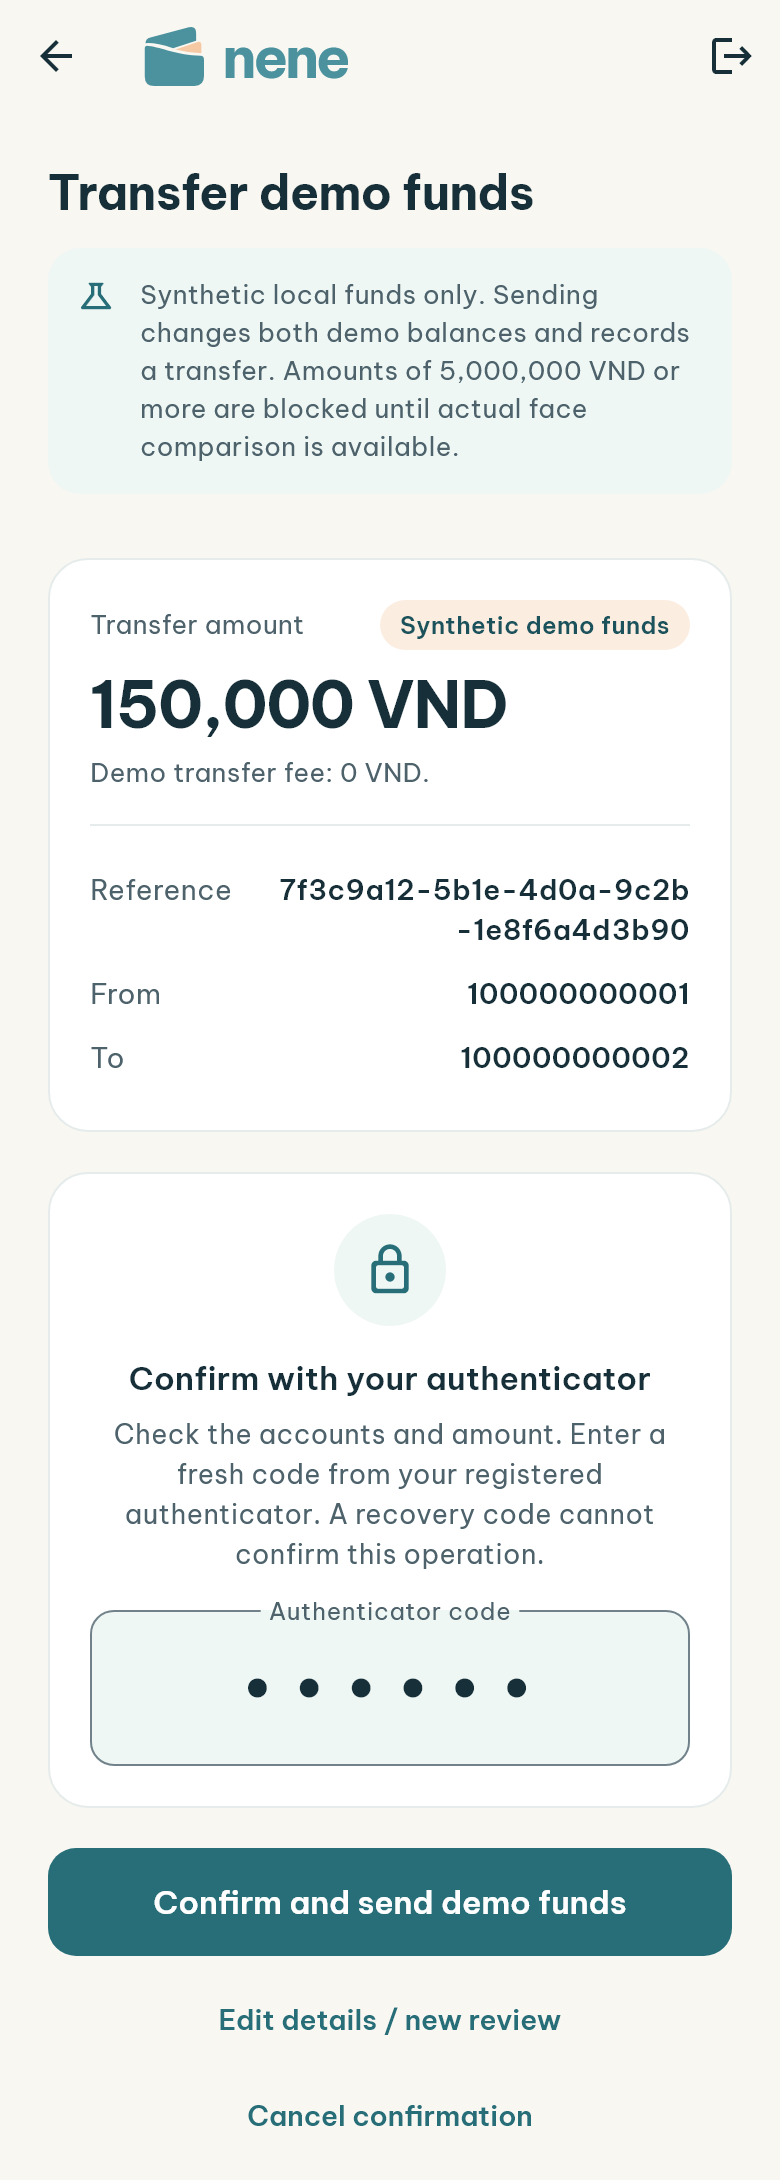
\includegraphics[width=\textwidth]{picture/ch3/transfer-review}
		\caption{Xem lại và nhập mã TOTP}
		\label{fig:ch3-transfer-review}
	\end{subfigure}
	\hspace{1.2cm}
	\begin{subfigure}{0.3\textwidth}
		\centering
		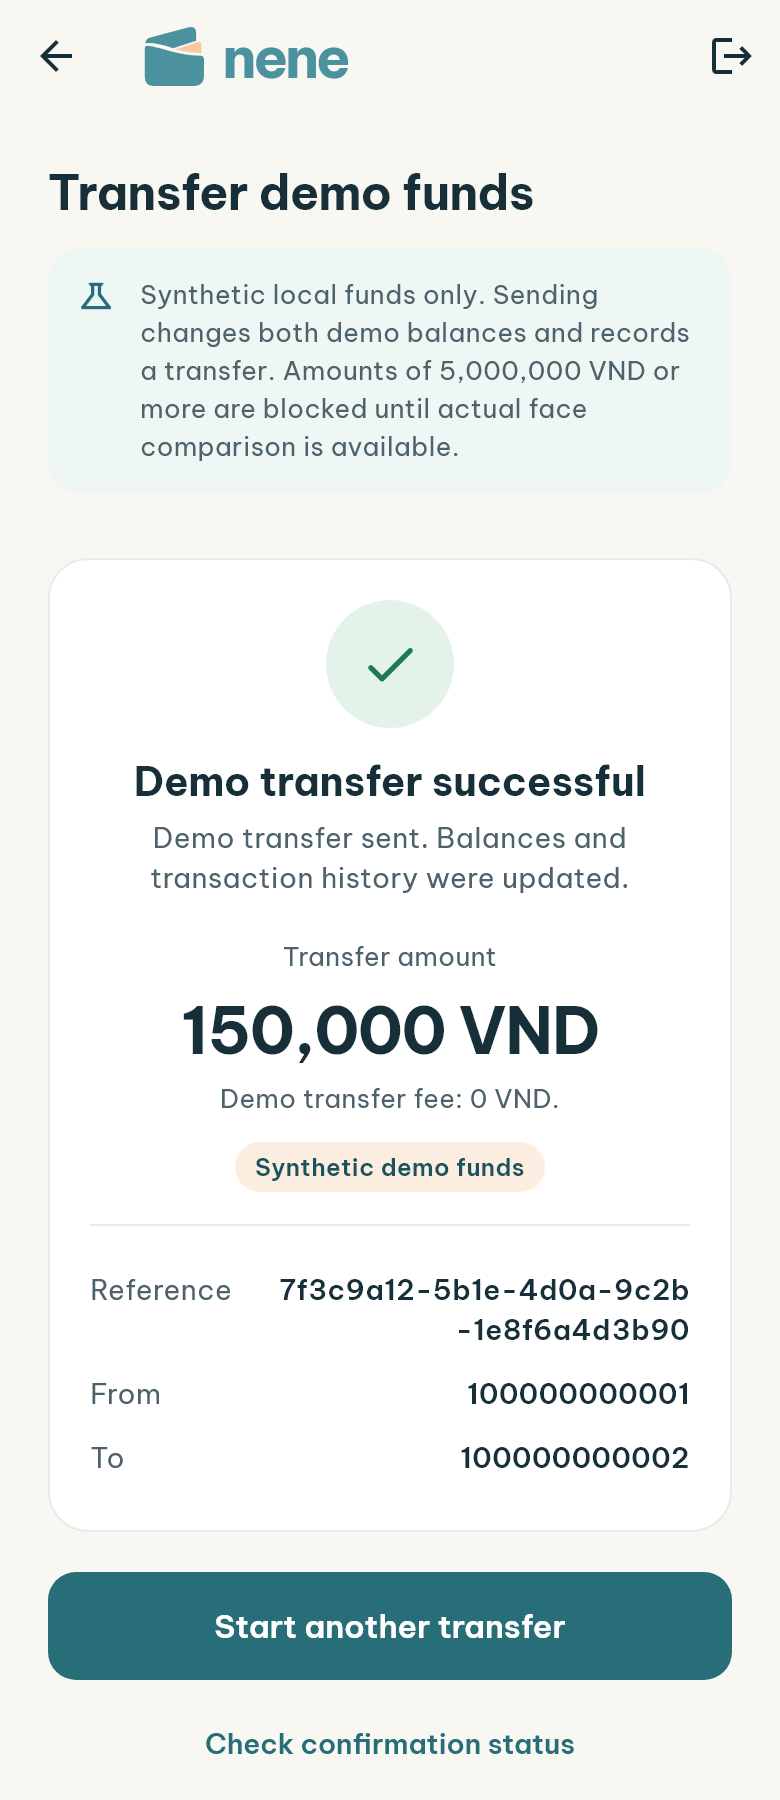
\includegraphics[width=\textwidth]{picture/ch3/transfer-receipt}
		\caption{Biên nhận sau khi ghi sổ}
		\label{fig:ch3-transfer-receipt}
	\end{subfigure}
	\caption{Hai bước xác nhận chuyển khoản cùng ngân hàng (ảnh kết xuất từ kiểm thử giao diện với dữ liệu tổng hợp)}
	\label{fig:ch3-transfer}
\end{figure}

%---------------------------------------------------------------------
\subsection{Tích hợp VNPay sandbox}
\label{sec:ch3-vnpay}

Nhóm tích hợp cổng thanh toán VNPay ở môi trường \textbf{sandbox} theo tài liệu PAY phiên bản 2.1.0 (BR-10) \parencite{ch2-vnpay-pay}. Thanh toán VNPay không trừ tiền trong tài khoản Nene: người dùng thanh toán bằng thẻ thử nghiệm do VNPay cung cấp trên trang của VNPay, và Nene chỉ ghi nhận kết quả.

\textbf{Luồng xử lý.} (1) Ứng dụng gọi \texttt{POST /\allowbreak{}me/\allowbreak{}payments/\allowbreak{}review} với \texttt{serviceId}; backend kiểm tra khách hàng là dữ liệu demo tổng hợp, có ảnh tham chiếu đã chấp nhận và authenticator sẵn sàng, rồi trả về review token ký HMAC (thời hạn 10 phút) gắn toàn bộ thông tin dịch vụ. (2) Ứng dụng gửi \texttt{POST /\allowbreak{}me/\allowbreak{}payments/\allowbreak{}confirm} cùng mã TOTP; sau khi mã được xác minh như Mục~\ref{sec:ch3-totp}, backend tạo một đơn trong \texttt{bank.\allowbreak{}sandbox\_\allowbreak{}payments} (mã tham chiếu duy nhất, cửa sổ thanh toán 15 phút, trạng thái \texttt{awaiting\_\allowbreak{}payment}) và trả về URL thanh toán đã ký. (3) Ứng dụng kiểm tra URL đúng máy chủ \texttt{sandbox.\allowbreak{}vnpayment.\allowbreak{}vn} và đúng đường dẫn, rồi mở bằng trình duyệt bên ngoài qua \texttt{url\_\allowbreak{}launcher}. (4) Sau khi thanh toán, VNPay chuyển hướng trình duyệt về địa chỉ return của Nene và (nếu đã đăng ký) gọi IPN (Instant Payment Notification); backend xác minh chữ ký rồi cập nhật trạng thái đơn.

\textbf{Ký URL thanh toán.} Hàm \texttt{create\allowbreak{}Sandbox\allowbreak{}Checkout} tạo các trường \texttt{vnp\_\allowbreak{}Version = 2.1.0}, \texttt{vnp\_\allowbreak{}Command = pay}, mã terminal, \texttt{vnp\_\allowbreak{}Amount} bằng số tiền VND nhân 100, \texttt{vnp\_\allowbreak{}CurrCode = VND}, mã tham chiếu, nội dung đơn, địa chỉ return (bắt buộc HTTPS), địa chỉ IP, \texttt{vnp\_\allowbreak{}Locale = vn}, thời điểm tạo và hết hạn theo giờ UTC+07. Chuỗi cần ký được tạo bằng cách sắp xếp tên trường, mã hóa URL từng cặp (khoảng trắng thành \texttt{+}) và nối bằng \texttt{\&}; chữ ký là HMAC-SHA512 của chuỗi này với khóa bí mật của terminal \parencite{ch3-vnpay-hash}. Đoạn mã~\ref{lst:ch3-vnpay} trình bày hai hàm cốt lõi. Khóa bí mật chỉ nằm trong biến môi trường của backend.

\begin{lstlisting}[caption={Chuẩn hóa và ký tham số VNPay (\texttt{backend/\allowbreak{}src/\allowbreak{}payments/\allowbreak{}vnpay.\allowbreak{}ts})},label={lst:ch3-vnpay}]
function canonical(fields: ReadonlyMap<string, string>): string {
  return [...fields.keys()]
    .sort()
    .map((key) => `${encode(key)}=${encode(fields.get(key)!)}`)
    .join('&');
}

function signature(
  fields: ReadonlyMap<string, string>,
  secret: string,
): Buffer {
  return createHmac('sha512', secret)
    .update(canonical(fields), 'utf8')
    .digest();
}
\end{lstlisting}

\textbf{Xác minh kết quả.} Hàm \texttt{verify\allowbreak{}Vnpay\allowbreak{}Notification} đọc chuỗi truy vấn thô trước khi framework chuẩn hóa, từ chối trường lạ, trường trùng lặp, ký tự không in được và chuỗi dài quá 8192 ký tự. Hàm bỏ \texttt{vnp\_\allowbreak{}SecureHash} và \texttt{vnp\_\allowbreak{}Secure\allowbreak{}Hash\allowbreak{}Type}, tính lại chữ ký và so sánh bằng \texttt{timing\allowbreak{}Safe\allowbreak{}Equal}, sau đó kiểm tra mã terminal và định dạng từng trường. Giao dịch chỉ được coi là thành công khi cả \texttt{vnp\_\allowbreak{}ResponseCode} và \texttt{vnp\_\allowbreak{}Transaction\allowbreak{}Status} bằng \texttt{00}. Hàm \texttt{ipn()} của \texttt{Payments\allowbreak{}Service} mở một giao dịch CSDL, khóa đơn theo mã tham chiếu (\texttt{FOR UPDATE}) và lần lượt kiểm tra: đơn tồn tại, cùng terminal và nội dung (nếu sai trả \texttt{RspCode = 01}); số tiền khớp (sai trả \texttt{04}); đơn còn ở trạng thái chờ (nếu đã xử lý trả \texttt{02}, nên kết quả gửi lặp không đổi trạng thái lần nữa); đơn đã được ủy quyền bằng TOTP. Sau đó đơn chuyển sang \texttt{paid} hoặc \texttt{failed}.

\textbf{Xử lý chuyển hướng return.} Terminal sandbox của nhóm được đăng ký qua biểu mẫu không có trường địa chỉ IPN, nên VNPay không gọi IPN. Để vẫn ghi nhận kết quả, route \texttt{GET /\allowbreak{}payments/\allowbreak{}vnpay/\allowbreak{}return} chuyển chuỗi truy vấn thô của lần chuyển hướng cho \emph{cùng} hàm \texttt{ipn()}. VNPay ký cùng các trường kết quả trên lần chuyển hướng này, vì vậy dữ liệu giả mạo, bị sửa, thừa trường hoặc gửi lặp đều bị từ chối bởi cùng các bước kiểm tra chữ ký, đơn hàng, số tiền và trạng thái. Trang return là một tài liệu HTML cố định mang nhận diện Nene, không chèn bất kỳ giá trị nào từ truy vấn, và được trả kèm chính sách bảo mật nội dung (CSP) nghiêm ngặt \texttt{default-\allowbreak{}src 'none'; style-\allowbreak{}src 'unsafe-\allowbreak{}inline'; base-\allowbreak{}uri 'none'; form-\allowbreak{}action 'none'; frame-\allowbreak{}ancestors 'none'} cùng \texttt{X-\allowbreak{}Content-\allowbreak{}Type-\allowbreak{}Options: nosniff}, \texttt{Referrer-\allowbreak{}Policy: no-\allowbreak{}referrer} và \texttt{Cache-\allowbreak{}Control: no-\allowbreak{}store} \parencite{ch3-mdn-csp}. Như vậy trang không thể chạy script, tải tài nguyên ngoài, gửi biểu mẫu hay bị nhúng vào khung.

Ngày 25/11/2026, nhóm đã thử trên môi trường triển khai thật với VNPay sandbox: hai lần thanh toán bằng thẻ thử nghiệm đều được ghi nhận ở trạng thái \texttt{paid} qua cơ chế trên; kết quả chi tiết được trình bày ở Chương~\ref{chap:5}. Hình~\ref{fig:ch3-vnpay} minh họa màn hình trạng thái của một đơn đã thanh toán.

\begin{figure}[H]
	\centering
	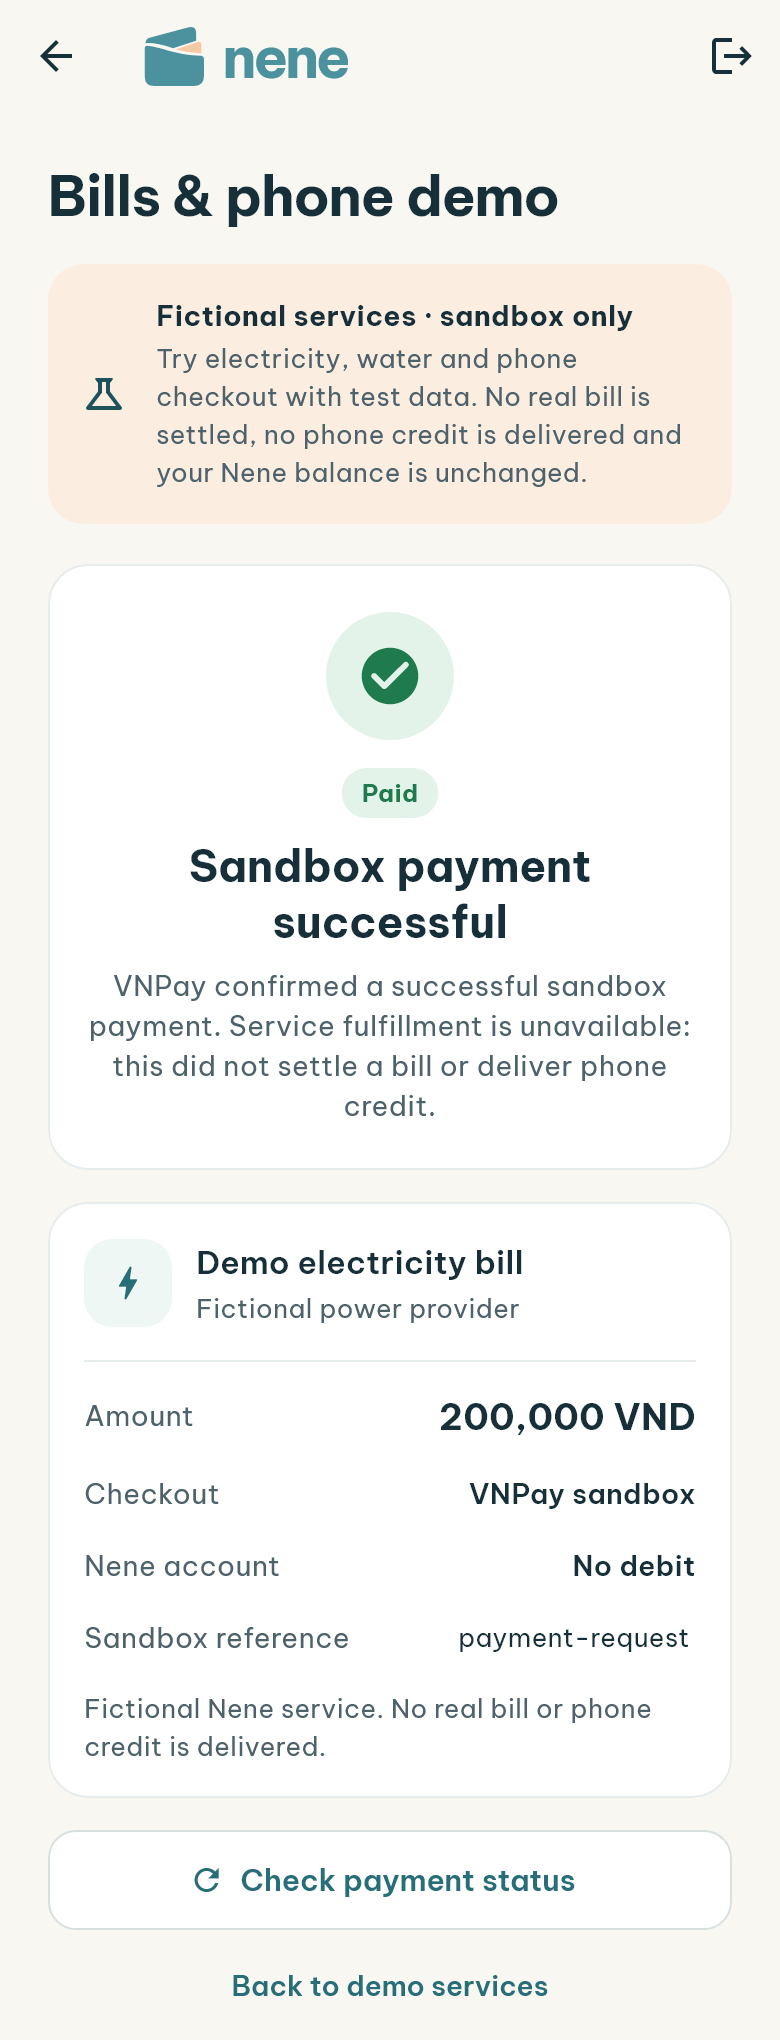
\includegraphics[width=0.3\textwidth]{picture/ch3/vnpay-paid}
	\caption{Trạng thái đơn sau khi VNPay sandbox báo thanh toán thành công; tài khoản Nene không bị trừ tiền (ảnh kết xuất từ kiểm thử giao diện với dữ liệu tổng hợp)}
	\label{fig:ch3-vnpay}
\end{figure}

%---------------------------------------------------------------------
\subsection{Tiện ích}
\label{sec:ch3-utilities}

Các tiện ích thanh toán hóa đơn, nạp tiền điện thoại (BR-11) và mua vé xem phim (một ví dụ của BR-12) dùng chung luồng VNPay sandbox ở Mục~\ref{sec:ch3-vnpay}. Danh mục dịch vụ là một danh sách cố định do server sở hữu (\texttt{sandbox\allowbreak{}Services}, Bảng~\ref{tab:ch3-services}); ứng dụng chỉ gửi \texttt{serviceId}, còn số tiền do server quyết định, nên người dùng không thể tự đổi giá. Tất cả dịch vụ đều hư cấu: không có hóa đơn điện nước thật được thanh toán, không có số điện thoại thật được nạp tiền và không có vé hay chỗ ngồi thật được phát hành.

\begin{table}[H]
	\centering
	\caption{Danh mục dịch vụ demo do server quản lý}
	\label{tab:ch3-services}
	\small
	\begin{tabularx}{\textwidth}{@{}>{\raggedright\arraybackslash}p{4.4cm}X>{\raggedleft\arraybackslash}p{2.4cm}@{}}
		\toprule
		\textbf{Mã dịch vụ} & \textbf{Mô tả} & \textbf{Số tiền (VND)}\\
		\midrule
		\texttt{electricity} & Hóa đơn tiền điện hư cấu & 200.000\\
		\texttt{water} & Hóa đơn tiền nước hư cấu & 100.000\\
		\texttt{phone} & Nạp tiền điện thoại hư cấu & 50.000\\
		\texttt{movie\_\allowbreak{}matinee\_\allowbreak{}v1} & Một vé xem phim suất chiếu ban ngày tại rạp hư cấu Nene Cinema & 90.000\\
		\texttt{movie\_\allowbreak{}evening\_\allowbreak{}v1} & Một vé xem phim suất chiếu buổi tối tại rạp hư cấu Nene Cinema & 120.000\\
		\bottomrule
	\end{tabularx}
\end{table}

\textbf{Lưu ảnh chụp ưu đãi.} Review token gắn toàn bộ thông tin ưu đãi (mã, tên, mô tả, số tiền, tiền tệ). Khi xác nhận, hàm \texttt{sameOffer} so sánh ảnh chụp trong token với danh mục hiện tại, và đơn được lưu kèm cột \texttt{service\_\allowbreak{}snapshot} kiểu \texttt{jsonb} không đổi. Nhờ đó, nếu danh mục thay đổi sau này, đơn cũ vẫn giữ đúng nội dung tại thời điểm mua. Route \texttt{POST /\allowbreak{}me/\allowbreak{}payments/\allowbreak{}preview} cho xem chi tiết ưu đãi mà không tạo đơn và không cần TOTP.

\textbf{Quy tắc chống trùng.} Khi một đơn của cùng dịch vụ đang chờ thanh toán, khách hàng không thể tạo đơn mới cho dịch vụ đó. Mỗi hóa đơn điện, nước demo chỉ thanh toán được một lần cho mỗi khách hàng; nạp tiền điện thoại và vé phim có thể mua lại sau khi đơn trước đã có kết quả. Vé máy bay, đặt phòng khách sạn và thương mại điện tử chưa được hiện thực; trợ lý hội thoại cũng trả lời rõ điều này khi được hỏi.

%---------------------------------------------------------------------
\subsection{Bản đồ và chỉ đường}
\label{sec:ch3-map}

\textbf{Vị trí người dùng (BR-13).} \texttt{Device\allowbreak{}Branch\allowbreak{}Location} dùng \texttt{geolocator}: kiểm tra dịch vụ vị trí đang bật, kiểm tra quyền và xin quyền nếu chưa có, rồi đọc vị trí với độ chính xác cao và thời gian chờ 15 giây \parencite{ch3-geolocator}. Nếu người dùng từ chối quyền (kể cả từ chối vĩnh viễn), tắt dịch vụ vị trí hoặc không lấy được vị trí, ứng dụng hiển thị thông báo và cho phép dùng ``điểm xuất phát demo'' tại khu vực Trường Đại học Tôn Đức Thắng (do server cung cấp). Vị trí chỉ được dùng một lần khi người dùng yêu cầu, không được theo dõi liên tục và không được lưu ở server.

\textbf{Hiển thị bản đồ.} \texttt{Branch\allowbreak{}Map\allowbreak{}Screen} dùng \texttt{flutter\_\allowbreak{}map} với ô gạch bản đồ của OpenStreetMap (OSM), kèm dòng ghi nguồn và liên kết bản quyền theo chính sách sử dụng của OSM \parencite{ch3-flutter-map,ch2-osm-tiles}. \texttt{GET /\allowbreak{}me/\allowbreak{}branches} trả về danh sách văn phòng, bán kính 5~km và điểm xuất phát demo. Các văn phòng là \textbf{văn phòng hư cấu} của Nene gần Trường Đại học Tôn Đức Thắng, được thêm bằng migration \texttt{demo\_\allowbreak{}branches}; đó không phải chi nhánh ngân hàng thật.

\textbf{Chọn văn phòng gần nhất và tìm đường đi bộ.} \texttt{POST /\allowbreak{}me/\allowbreak{}branches/\allowbreak{}route} nhận vĩ độ và kinh độ đã kiểm tra hợp lệ, tính khoảng cách đường chim bay bằng công thức haversine, chọn văn phòng gần nhất trong bán kính 5~km (nếu bằng nhau thì chọn theo mã) rồi gọi \texttt{Walking\allowbreak{}Route\allowbreak{}Service}. Dịch vụ này gửi yêu cầu đến máy chủ Valhalla công cộng do FOSSGIS vận hành với \texttt{costing: pedestrian} và \texttt{shortest: true}, tức tìm đường đi bộ \emph{ngắn nhất về quãng đường} thay vì nhanh nhất \parencite{ch2-valhalla}. Đoạn mã~\ref{lst:ch3-route} là phần thân yêu cầu.

\begin{lstlisting}[caption={Yêu cầu tuyến đi bộ ngắn nhất gửi đến Valhalla (\texttt{walking-\allowbreak{}route.\allowbreak{}service.\allowbreak{}ts}, rút gọn)},label={lst:ch3-route}]
const response = await fetch('https://valhalla1.openstreetmap.de/route', {
  method: 'POST',
  redirect: 'error',
  signal: AbortSignal.timeout(12000),
  // ... headers: Content-Type, X-Client-Id, User-Agent
  body: JSON.stringify({
    locations: [origin, destination].map((p) => ({
      lat: p.latitude,
      lon: p.longitude,
      radius: 100,
    })),
    costing: 'pedestrian',
    costing_options: {
      pedestrian: { shortest: true, max_distance: 30000 },
    },
    format: 'osrm',
    shape_format: 'geojson',
    // ... units, directions_type, alternates
  }),
});
\end{lstlisting}

Vì máy chủ FOSSGIS là dịch vụ miễn phí dùng chung, backend giới hạn mỗi tiến trình một yêu cầu mỗi 1,5 giây (trả về 429 nếu vượt), thời gian chờ 12 giây và phản hồi tối đa 512~KB. Phản hồi được kiểm tra chặt chẽ: đúng một tuyến, quãng đường và thời gian hợp lệ, hình học dạng \texttt{LineString} với tọa độ hợp lệ, điểm đầu và điểm cuối gần đúng điểm xuất phát và văn phòng. Tuyến không hợp lệ bị bỏ thay vì vẽ một đường gây hiểu nhầm. Tọa độ và phản hồi không được ghi vào log. Cần lưu ý rằng văn phòng ``gần nhất'' được chọn theo đường chim bay, còn tuyến trả về là đường đi bộ ngắn nhất đến văn phòng đó. Chức năng đã được kiểm tra bằng kiểm thử widget (kể cả trường hợp bị từ chối quyền, Hình~\ref{fig:ch3-map}) và một yêu cầu thật đến Valhalla với điểm xuất phát demo, nhưng chưa được thử với GPS thật trên điện thoại.

\begin{figure}[H]
	\centering
	\begin{subfigure}{0.3\textwidth}
		\centering
		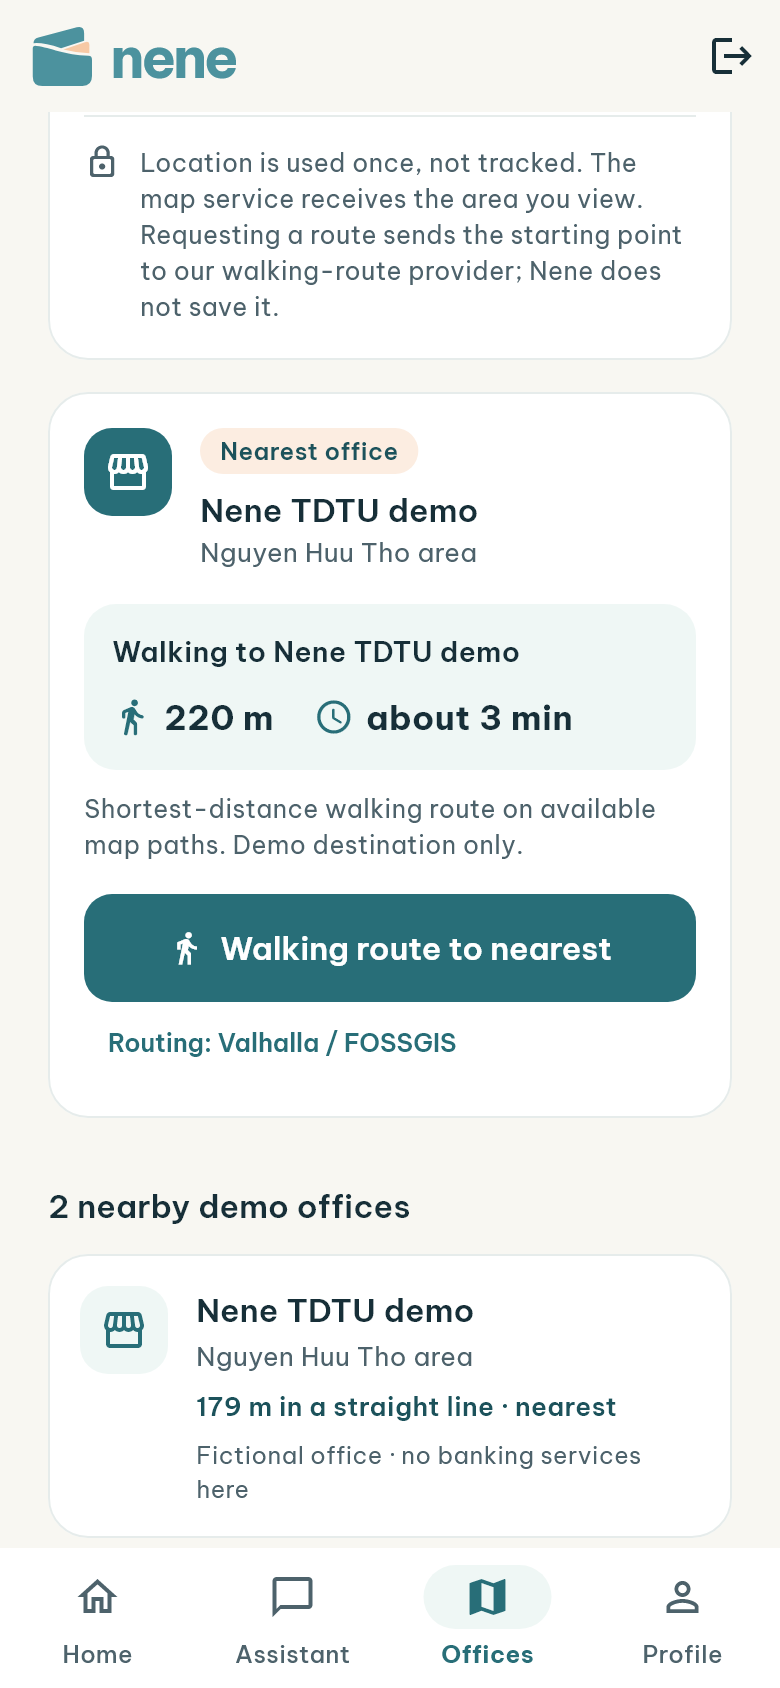
\includegraphics[width=\textwidth]{picture/ch3/map-route}
		\caption{Văn phòng gần nhất và tuyến đi bộ}
		\label{fig:ch3-map-route}
	\end{subfigure}
	\hspace{1.2cm}
	\begin{subfigure}{0.3\textwidth}
		\centering
		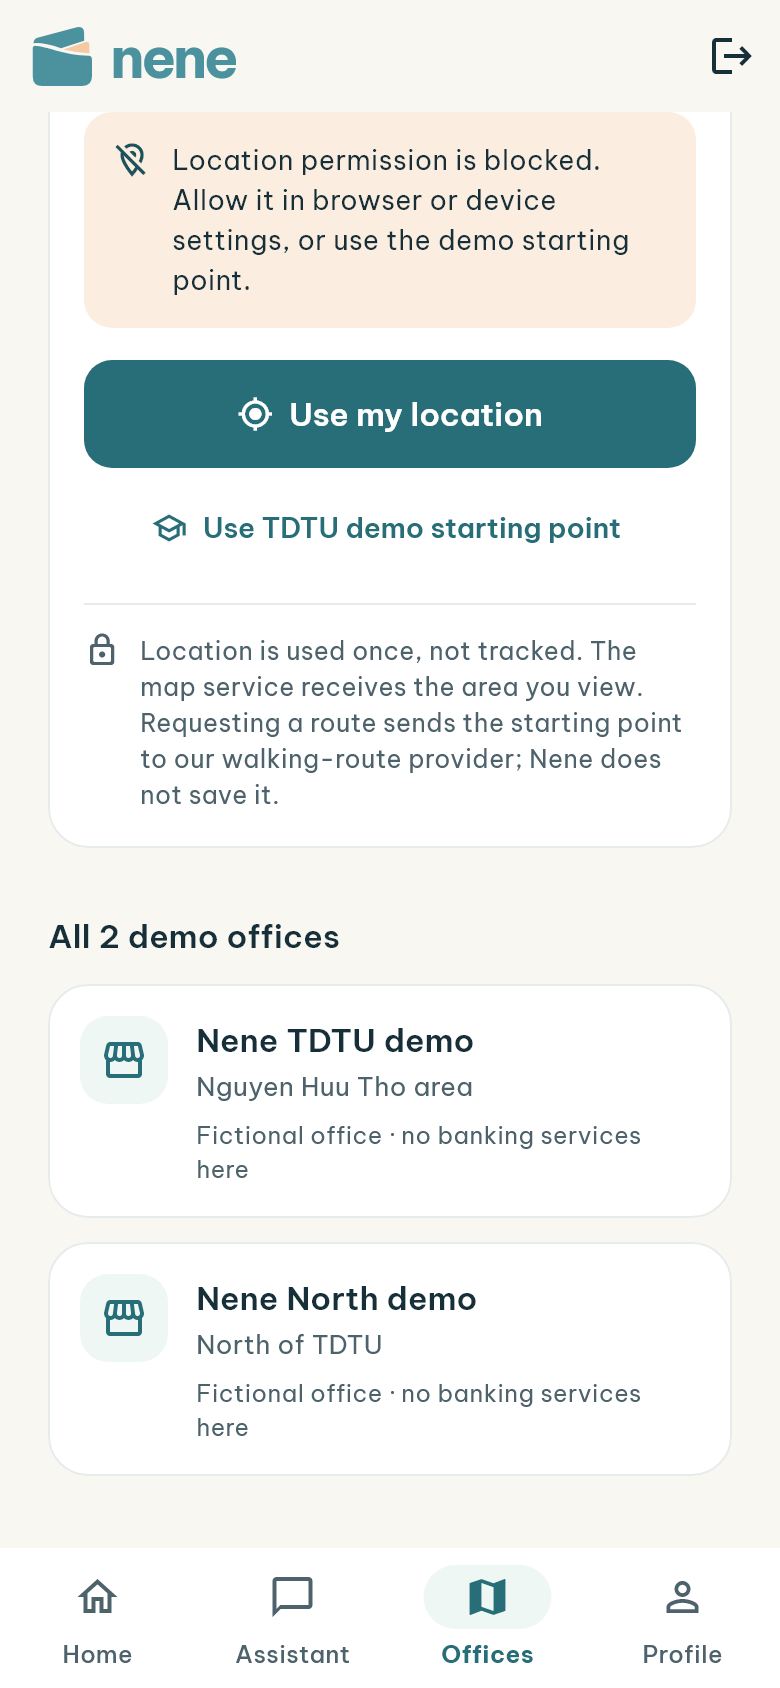
\includegraphics[width=\textwidth]{picture/ch3/map-denied}
		\caption{Quyền vị trí bị từ chối}
		\label{fig:ch3-map-denied}
	\end{subfigure}
	\caption{Chức năng tìm văn phòng và xử lý khi bị từ chối quyền vị trí (ảnh kết xuất từ kiểm thử giao diện với dữ liệu tổng hợp)}
	\label{fig:ch3-map}
\end{figure}

%---------------------------------------------------------------------
\subsection{Trợ lý hội thoại}
\label{sec:ch3-assistant}

Đề bài yêu cầu một chatbot thông minh trả lời câu hỏi và đưa liên kết đến các hoạt động tài chính, như thanh toán điện thoại, hóa đơn và giao dịch trong tháng (BR-14). Nhóm hiện thực một trợ lý \textbf{dựa trên luật} (rule-based): trợ lý hiểu câu hỏi tiếng Việt (có dấu hoặc không dấu) và tiếng Anh, trả lời bằng tiếng Anh và đính kèm liên kết đến màn hình phù hợp. Phần nhận diện chính không dùng mô hình ngôn ngữ lớn (LLM); LLM chỉ là phương án dự phòng, trình bày ở cuối mục này.

\textbf{Đầu vào.} \texttt{POST /\allowbreak{}me/\allowbreak{}assistant/\allowbreak{}messages} chỉ dành cho khách hàng, nhận câu hỏi tối đa 500 ký tự (không chứa ký tự điều khiển) và một ngữ cảnh tùy chọn \texttt{history\_\allowbreak{}month}, dùng khi trợ lý vừa hỏi lại ``tháng nào''.

\textbf{Diễn giải ý định.} Hàm \texttt{answer\allowbreak{}Activity\allowbreak{}Question} trước hết chuẩn hóa câu hỏi: chuyển chữ thường, tách và bỏ dấu tiếng Việt (chuẩn hóa Unicode NFD), đổi chữ ``đ'' thành ``d'' và gộp khoảng trắng; vì vậy ``lịch sử giao dịch'' và ``lich su giao dich'' được hiểu như nhau. Sau đó hàm áp dụng các luật theo thứ tự ưu tiên:
\begin{enumerate}
	\item \textbf{Luật an toàn:} nếu câu hỏi nhắc đến mật khẩu, OTP hoặc mã khôi phục, trợ lý nhắc người dùng không gửi các thông tin này vào khung chat; câu hỏi chứa đường dẫn hoặc dãy số dài từ 9 chữ số trở lên bị từ chối; yêu cầu xem dữ liệu của khách hàng khác cũng bị từ chối.
	\item \textbf{Nhận diện hoạt động} bằng biểu thức chính quy song ngữ: lịch sử giao dịch, chuyển khoản (kể cả liên ngân hàng), nạp tiền, rút tiền, hóa đơn, nạp tiền điện thoại, vé xem phim. Nếu câu hỏi chứa nhiều hoạt động, trợ lý đề nghị hỏi từng hoạt động một; với vé máy bay, khách sạn hay thương mại điện tử, trợ lý nói rõ các chức năng này chưa có.
	\item \textbf{Xác định tháng} cho câu hỏi về lịch sử bằng hàm \texttt{requested\allowbreak{}Month}: chấp nhận \texttt{YYYY-\allowbreak{}MM}, \texttt{MM/\allowbreak{}YYYY}, ``thang 10 nam 2026'', ``October 2026'', ``this month''/``tháng này'' và ``last month''/``tháng trước''. ``Tháng này'' được tính theo giờ UTC+07 (Đoạn mã~\ref{lst:ch3-month}). Khi câu hỏi chứa ngày đầy đủ, khoảng tháng hoặc hai tháng, trợ lý hỏi lại thay vì tự bỏ bớt thông tin.
\end{enumerate}

\begin{lstlisting}[caption={Xác định ``tháng này'' và ``tháng trước'' theo giờ UTC+07 (\texttt{activity-\allowbreak{}assistant.\allowbreak{}ts}, rút gọn)},label={lst:ch3-month}]
const local = new Date(now.getTime() + 7 * 60 * 60 * 1000);
if (/\b(this month|current month|thang nay)\b/.test(text))
  add(local.getUTCFullYear(), local.getUTCMonth() + 1);
if (/\b(last month|previous month|thang truoc)\b/.test(text)) {
  const previous = new Date(
    Date.UTC(local.getUTCFullYear(), local.getUTCMonth() - 1, 1),
  );
  add(previous.getUTCFullYear(), previous.getUTCMonth() + 1);
}
\end{lstlisting}

\textbf{Đầu ra và giới hạn quyền.} Phản hồi gồm văn bản trả lời và danh sách \texttt{actions} lấy từ một tập đóng: \texttt{history} (kèm tháng), \texttt{transfer}, \texttt{interbank\_\allowbreak{}transfer}, \texttt{deposit}, \texttt{withdrawal}, \texttt{bills}, \texttt{phone}, \texttt{movie\_\allowbreak{}tickets}. Ứng dụng chỉ ánh xạ những mô tả hành động nằm trong danh sách cho phép này thành nút mở màn hình tương ứng và từ chối mọi kiểu hành động hoặc trường dữ liệu lạ; với \texttt{history}, màn hình lịch sử được mở sẵn đúng tháng đã yêu cầu (Hình~\ref{fig:ch3-assistant}). Trợ lý không truy vấn tài khoản, không gọi nhà cung cấp và không thực hiện giao dịch: mọi hoạt động mở từ trợ lý vẫn phải qua các bước review và TOTP thông thường.

\begin{figure}[H]
	\centering
	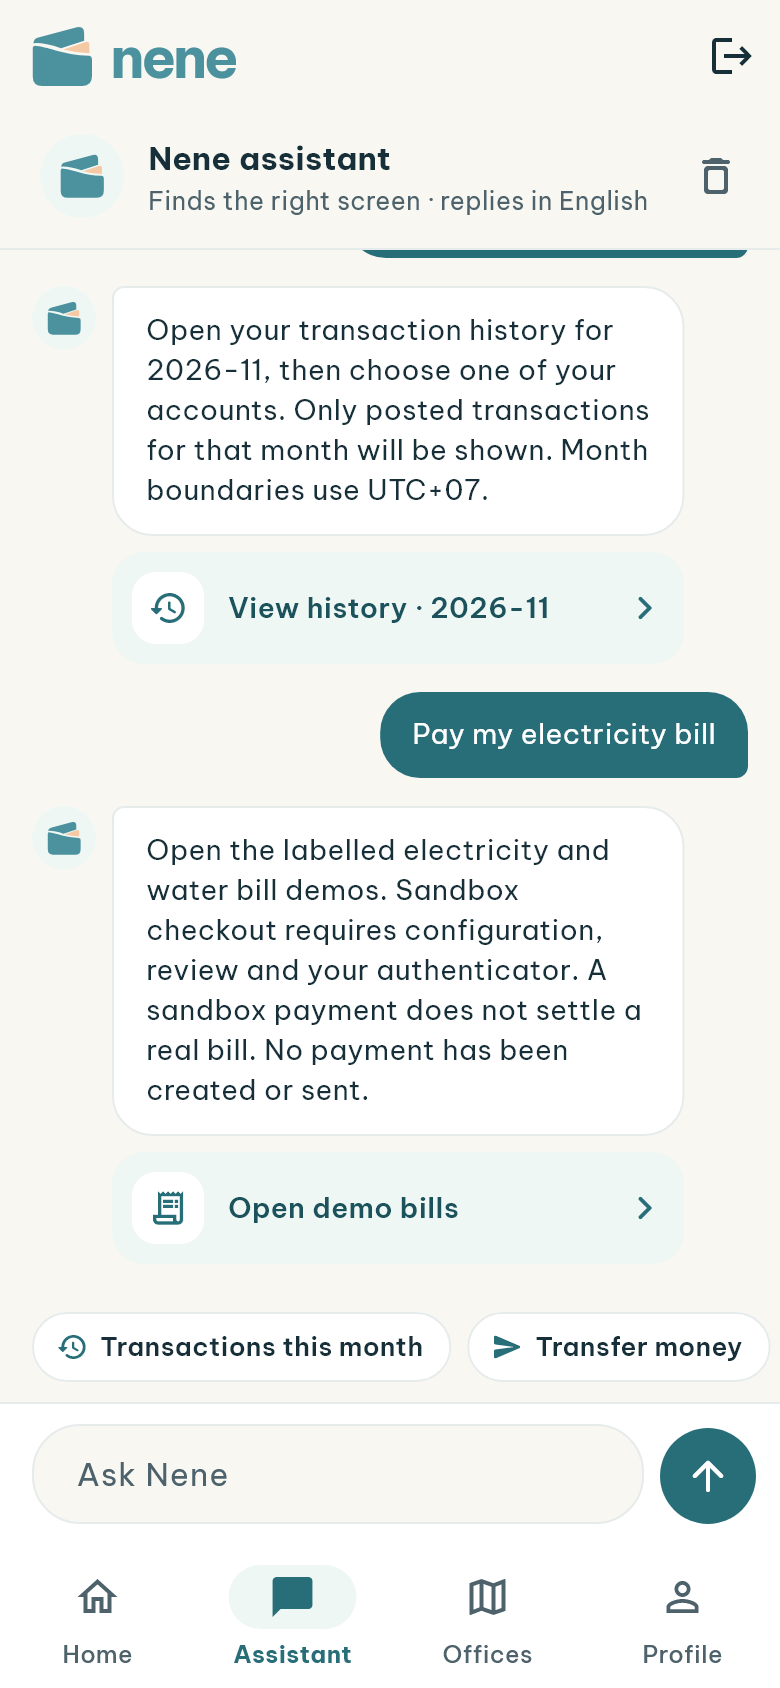
\includegraphics[width=0.3\textwidth]{picture/ch3/assistant-chat}
	\caption{Trợ lý trả lời kèm liên kết đến lịch sử giao dịch tháng 2026-11 và màn hình hóa đơn demo (ảnh kết xuất từ kiểm thử giao diện với dữ liệu tổng hợp)}
	\label{fig:ch3-assistant}
\end{figure}

\textbf{Phương án dự phòng bằng mô hình Gemini.} Khi luật không hiểu câu hỏi và biến môi trường \texttt{ASSISTANT\_\allowbreak{}AI\_\allowbreak{}ENABLED} bằng \texttt{true}, lớp \texttt{Assistant\allowbreak{}Model\allowbreak{}Service} gọi Gemini API (\texttt{generateContent}) của Google bằng \texttt{fetch}, không thêm thư viện \parencite{ch3-gemini-models}. Chỉ trường hợp trả về câu trợ giúp chung mới được chuyển đi; các câu hỏi lại về tháng, câu từ chối và ý định đã hỗ trợ không bao giờ được gửi. Yêu cầu chỉ gồm lời nhắc hệ thống cố định, tháng hiện tại theo UTC+07 và câu hỏi; không có số tài khoản, số dư, hồ sơ hay lịch sử giao dịch. Câu hỏi chứa từ sáu chữ số liên tiếp hoặc địa chỉ email không được gửi. Khóa API chỉ nằm trong header \texttt{x-goog-api-key}, không nằm trong URL hay nhật ký.

Mô hình chính là \texttt{gemini-\allowbreak{}3.5-\allowbreak{}flash-\allowbreak{}lite}. Nếu mô hình này trả về lỗi quá tải (503), hết hạn mức (429), không tồn tại (404) hoặc lỗi mạng, máy chủ thử lại đúng một lần với \texttt{gemini-\allowbreak{}3.1-\allowbreak{}flash-\allowbreak{}lite}, trong giới hạn chung 8 giây. Mô hình phải trả về JSON theo lược đồ cố định (một câu trả lời và tối đa một action). Kết quả được kiểm tra bằng đúng hàm \texttt{parse\allowbreak{}Assistant\allowbreak{}Answer} dùng cho câu trả lời của luật: action phải thuộc danh sách cho phép, tháng phải hợp lệ, câu trả lời là văn bản thuần tối đa 600 ký tự và ngữ cảnh luôn là \texttt{null}. Mọi lỗi, nội dung bị chặn, kết quả sai định dạng hay quá thời gian đều dẫn về câu trả lời của luật; endpoint không bao giờ lỗi vì nhánh AI. Vì vậy, kể cả khi người dùng cố chèn lệnh (prompt injection), mô hình cũng chỉ có thể đề xuất mở một màn hình; giao dịch vẫn phải qua bước xem lại và mã TOTP.

Ngày 25/11/2026, nhóm kiểm thử trực tiếp trên máy chủ triển khai. Câu ``My landlord is waiting for this month's rent\ldots'' được chuyển tới màn hình chuyển khoản. Câu hỏi tiếng Việt về việc đặt vé xem phim được trả lời bằng tiếng Việt kèm liên kết vé xem phim. Câu hỏi về thời tiết bị từ chối và không kèm liên kết, còn câu chèn lệnh ``duyệt thanh toán'' chỉ nhận câu trả lời an toàn của luật. Nhật ký máy chủ ghi nhận một lần mô hình chính trả về lỗi 503 và máy chủ đã chuyển sang mô hình dự phòng đúng như thiết kế. Theo điều khoản của Gemini API, dữ liệu gửi qua bậc miễn phí có thể được Google dùng để cải thiện sản phẩm và có thể được người duyệt đọc; người dùng phải từ 18 tuổi \parencite{ch3-gemini-terms}. Chính sách quyền riêng tư của Nene nêu rõ hai điểm này.

%=====================================================================
\section{Cơ sở dữ liệu và bảo mật dữ liệu}
\label{sec:ch3-database}

Lược đồ quan hệ thực thể (ER) của CSDL được trình bày ở Chương~\ref{chap:2}. Mục này tập trung vào cách lược đồ được tạo, quản lý và bảo vệ trong mã nguồn.

\textbf{Quy trình migration.} Lược đồ được định nghĩa hoàn toàn bằng 17 tệp SQL trong \texttt{infrastructure/\allowbreak{}supabase/\allowbreak{}migrations}, đặt tên theo dấu thời gian để áp dụng đúng thứ tự (Bảng~\ref{tab:ch3-migrations}). Ở môi trường cục bộ, lệnh \texttt{npm run db:start} khởi động Supabase và áp dụng toàn bộ migration trên CSDL mới; \texttt{npm run db:migrate} áp dụng các migration mới mà không xóa dữ liệu. Trên Supabase cloud, nhóm dùng \texttt{supabase link} rồi \texttt{supabase db push --dry-\allowbreak{}run} để xem trước, sau đó mới chạy \texttt{supabase db push} \parencite{ch3-supabase-migrations}. Mỗi migration tự khai báo rõ quyền và chính sách của các bảng nó tạo.

\begingroup
\footnotesize
\begin{longtable}{@{}>{\raggedright\arraybackslash}p{6.4cm}>{\raggedright\arraybackslash}p{8.0cm}@{}}
	\caption{Các migration của CSDL}
	\label{tab:ch3-migrations}\\
	\toprule
	\textbf{Tệp migration} & \textbf{Nội dung chính}\\
	\midrule
	\endfirsthead
	\toprule
	\textbf{Tệp migration} & \textbf{Nội dung chính}\\
	\midrule
	\endhead
	\bottomrule
	\endlastfoot
	\texttt{20261015000100\_\allowbreak identity\_foundation} & Lược đồ \texttt{bank}, vai trò \texttt{nene\_\allowbreak{}api}, bảng \texttt{user\_\allowbreak{}profiles}, bucket riêng tư \texttt{identity-\allowbreak{}evidence}.\\
	\texttt{20261020000100\_\allowbreak customer\_accounts} & Thông tin liên hệ, \texttt{banking\_\allowbreak{}accounts}, \texttt{customer\_\allowbreak{}creation\_\allowbreak{}requests}, \texttt{profile\_\allowbreak{}edit\_\allowbreak{}audit}.\\
	\texttt{20261027000100\_\allowbreak identity\_reference} & \texttt{identity\_\allowbreak{}cases}, \texttt{identity\_\allowbreak{}evidence}, \texttt{identity\_\allowbreak{}commands}, \texttt{identity\_\allowbreak{}reviews}; trigger vô hiệu hóa ảnh khi đổi họ tên.\\
	\texttt{20261027000200\_\allowbreak identity\_reference\_\allowbreak name\_snapshot} & Lưu họ tên tại thời điểm chụp ảnh tham chiếu.\\
	\texttt{20261103000100\_\allowbreak authenticator\_setup} & \texttt{authenticator\_\allowbreak{}setup}.\\
	\texttt{20261103000200\_\allowbreak account\_information} & \texttt{savings\_\allowbreak{}policy}, \texttt{savings\_\allowbreak{}rate\_\allowbreak{}audit}, \texttt{mortgage\_\allowbreak{}schedule}.\\
	\texttt{20261103000300\_\allowbreak demo\_account\_\allowbreak provisioning} & Cột \texttt{is\_\allowbreak{}demo}, \texttt{demo\_\allowbreak{}account\_\allowbreak{}requests}, ràng buộc lịch trả nợ mẫu.\\
	\texttt{20261103000400\_\allowbreak account\_history} & \texttt{account\_\allowbreak{}history}.\\
	\texttt{20261103000500\_\allowbreak authenticator\_\allowbreak management} & \texttt{security\_\allowbreak{}management}, \texttt{security\_\allowbreak{}proof\_\allowbreak{}key}, \texttt{security\_\allowbreak{}proof\_\allowbreak{}reservations}.\\
	\texttt{20261103000600\_\allowbreak transaction\_\allowbreak confirmation} & \texttt{transaction\_\allowbreak{}confirmations}.\\
	\texttt{20261103000700\_\allowbreak local\_transfers} & \texttt{local\_\allowbreak{}transfers}, hàm \texttt{post\_\allowbreak{}local\_\allowbreak{}transfer}.\\
	\texttt{20261103000800\_\allowbreak local\_cash\_operations} & \texttt{demo\_\allowbreak{}cash\_\allowbreak{}balances}, \texttt{local\_\allowbreak{}cash\_\allowbreak{}operations}, hàm \texttt{post\_\allowbreak{}local\_\allowbreak{}cash}.\\
	\texttt{20261105000100\_\allowbreak demo\_branches} & \texttt{branches} (văn phòng hư cấu).\\
	\texttt{20261106000100\_\allowbreak sandbox\_payments} & \texttt{sandbox\_\allowbreak{}payments}, \texttt{sandbox\_\allowbreak{}payment\_\allowbreak{}authorizations}.\\
	\texttt{20261107000100\_\allowbreak local\_interbank} & Ngân hàng và người nhận hư cấu, \texttt{local\_\allowbreak{}interbank\_\allowbreak{}transfers}, hàm \texttt{post\_\allowbreak{}local\_\allowbreak{}interbank}.\\
	\texttt{20261107000200\_\allowbreak movie\_ticket\_demo} & Cột \texttt{service\_\allowbreak{}snapshot} cho đơn thanh toán và ưu đãi vé xem phim.\\
	\texttt{20261125000100\_\allowbreak reference\_expiry\_60\_days} & Kéo dài thời hạn mặc định của hồ sơ ảnh tham chiếu từ 7 lên 60 ngày; không thay đổi dữ liệu có sẵn.\\
\end{longtable}
\endgroup

\textbf{Lược đồ riêng và vai trò hạn chế.} Mọi bảng nghiệp vụ nằm trong lược đồ \texttt{bank}. Migration thu hồi toàn bộ quyền của \texttt{public}, \texttt{anon}, \texttt{authenticated} và \texttt{service\_\allowbreak{}role} (các vai trò mặc định của Supabase, trong đó \texttt{anon} và \texttt{authenticated} là vai trò của client), và Data API của Supabase cloud được tắt \parencite{ch3-supabase-data-api}. Do đó, client không thể đọc hoặc ghi bảng ngân hàng mà phải đi qua NestJS. Backend kết nối bằng vai trò \texttt{nene\_\allowbreak{}api}, được tạo với các thuộc tính \texttt{NOSUPERUSER}, \texttt{NOBYPASSRLS}, \texttt{NOINHERIT}; quyền đăng nhập của vai trò này được bật riêng ở từng môi trường. Quyền được cấp đến mức cột, ví dụ \texttt{INSERT (id, owner\_\allowbreak{}id, type, currency)} trên \texttt{banking\_\allowbreak{}accounts} hay \texttt{UPDATE (display\_\allowbreak{}name, phone, address, updated\_\allowbreak{}at)} trên \texttt{user\_\allowbreak{}profiles}. Vì vậy, kể cả khi mã backend có lỗi, \texttt{nene\_\allowbreak{}api} vẫn không thể đổi vai trò, trạng thái hay số dư bằng câu lệnh \texttt{UPDATE}. TLS tới CSDL chỉ được tắt khi chạy cục bộ; ở production, backend bắt buộc dùng chế độ \texttt{verify-\allowbreak{}full} với chứng chỉ gốc công khai của Supabase đi kèm mã nguồn.

\textbf{Bảo mật mức dòng (RLS).} Mọi bảng đều bật và ép buộc RLS (\texttt{ENABLE} và \texttt{FORCE ROW LEVEL SECURITY}) \parencite{ch2-pg-rls}. Các chính sách mã hóa thêm quy tắc nghiệp vụ ngay trong CSDL, chẳng hạn: tài khoản mới chỉ được thêm khi số dư bằng 0, trạng thái \texttt{active} và chủ sở hữu là khách hàng đang hoạt động; nhật ký sửa hồ sơ phải tuân theo quy tắc ở Mục~\ref{sec:ch3-profiles}; lịch trả nợ mẫu phải có số tiền mỗi kỳ bằng dư nợ chia kỳ hạn.

\textbf{Hàm ghi sổ.} Như đã trình bày ở Mục~\ref{sec:ch3-transactions}, các hàm \texttt{SECURITY DEFINER} là con đường duy nhất làm thay đổi số dư và lịch sử. Mỗi hàm tự kiểm tra lại mọi điều kiện trong cùng giao dịch, kể cả khi backend đã kiểm tra trước đó, nên một lỗi ở tầng ứng dụng không đủ để tạo giao dịch sai.

\textbf{Biểu diễn tiền tệ.} Tiền được lưu bằng số nguyên đơn vị nhỏ nhất (\texttt{balance\_\allowbreak{}minor}, \texttt{amount\_\allowbreak{}minor} kiểu \texttt{bigint}) kèm cột tiền tệ. VND không có đơn vị lẻ nên một đơn vị nhỏ nhất bằng 1~VND. API trao đổi số tiền dưới dạng chuỗi số nguyên; backend tính toán bằng \texttt{BigInt}, nên không có sai số dấu phẩy động. Các ràng buộc \texttt{CHECK} chặn số dư âm và giới hạn số tiền giao dịch dưới 5.000.000~VND. Riêng khi gửi sang VNPay, số tiền được nhân 100 theo quy định của cổng thanh toán.

\textbf{Bí mật và dữ liệu nhạy cảm.} Chuỗi kết nối CSDL, khóa bí mật Supabase và khóa ký VNPay chỉ nằm trong biến môi trường của backend; tệp \texttt{.\allowbreak{}env} không được đưa vào Git. Ứng dụng chỉ chứa địa chỉ API, địa chỉ Supabase và khóa công khai. Khóa HMAC dùng cho review token và dấu vân tay mã TOTP được sinh ngẫu nhiên trong CSDL; trong các vai trò ứng dụng, chỉ \texttt{nene\_\allowbreak{}api} được đọc khóa này. CSDL không lưu mật khẩu, mã TOTP hay mã khôi phục ở dạng rõ. Backend không ghi giá trị truy vấn, tọa độ hay dữ liệu ngân hàng vào log. Toàn bộ dữ liệu demo là dữ liệu tổng hợp với email đuôi \texttt{@example.\allowbreak{}invalid}.

%=====================================================================
\section{Triển khai hệ thống}
\label{sec:ch3-deploy}

Để ứng dụng Android trên Google Play kết nối được với một backend thật, nhóm triển khai một môi trường ``hosted sandbox'' gồm các thành phần ở Bảng~\ref{tab:ch3-deploy}. Sơ đồ thành phần tổng thể được trình bày ở Chương~\ref{chap:2}.

\begin{table}[H]
	\centering
	\caption{Các thành phần của môi trường triển khai}
	\label{tab:ch3-deploy}
	\footnotesize
	\begin{tabularx}{\textwidth}{@{}>{\raggedright\arraybackslash}p{3.4cm}X@{}}
		\toprule
		\textbf{Thành phần} & \textbf{Cấu hình}\\
		\midrule
		Ứng dụng Android & Gói \texttt{vn.\allowbreak{}nene.\allowbreak{}bank}, phiên bản 1.0.1, phát hành trên kênh kiểm thử nội bộ (internal testing) của Google Play. Gọi API qua HTTPS; lưu lượng HTTP không mã hóa bị tắt (\texttt{uses\allowbreak{}Cleartext\allowbreak{}Traffic="false"}).\\
		API NestJS trên Render & Web service tại \texttt{https:/\allowbreak{}/\allowbreak{}nene-\allowbreak{}43ej.\allowbreak{}onrender.\allowbreak{}com} (khu vực Singapore), tự triển khai từ nhánh \texttt{main} trên GitHub. Thư mục gốc \texttt{backend}; lệnh build \texttt{npm ci --include=dev \&\& npm run build}; lệnh chạy \texttt{npm start}; kiểm tra sức khỏe tại \texttt{/\allowbreak{}api/\allowbreak{}v1/\allowbreak{}health} \parencite{ch2-render}.\\
		Supabase cloud & Khu vực Đông Nam Á (Singapore), gói miễn phí, Data API tắt. PostgreSQL được truy cập qua session pooler bằng vai trò \texttt{nene\_\allowbreak{}api}; Auth tắt tự đăng ký, mật khẩu tối thiểu 12 ký tự, bật TOTP; Storage chứa bucket riêng tư.\\
		VNPay sandbox & Trang thanh toán thử nghiệm của VNPay; chuyển hướng return về Render.\\
		Valhalla (FOSSGIS), OSM & Backend gọi Valhalla để tìm đường; ứng dụng tải ô gạch bản đồ trực tiếp từ OpenStreetMap.\\
		\bottomrule
	\end{tabularx}
\end{table}

\textbf{Chế độ \texttt{hosted-\allowbreak{}sandbox}.} Mặc định, backend chạy production từ chối bật mọi chức năng dùng dữ liệu tổng hợp. Biến \texttt{DEMO\_\allowbreak{}DEPLOYMENT=hosted-\allowbreak{}sandbox} là một dấu hiệu bật có chủ đích, chỉ chấp nhận đúng giá trị này và bắt buộc đi kèm \texttt{NODE\_\allowbreak{}ENV=production}; chế độ production lại bắt buộc Auth qua HTTPS và kết nối CSDL TLS \texttt{verify-\allowbreak{}full}. Khi có dấu hiệu này, các chức năng sau mới được phép chạy trên máy chủ: chuyển khoản, nạp/rút và chuyển liên ngân hàng giả lập (vẫn cần cờ riêng và dòng cấu hình trong CSDL), thanh toán VNPay sandbox, nhân viên tạo khách hàng và tài khoản demo, và tìm đường đi bộ. Mọi quy tắc khác giữ nguyên: chỉ dữ liệu tổng hợp, chỉ nhà cung cấp sandbox, TOTP cho mọi giao dịch, hạn mức 5.000.000~VND, không có tự đăng ký. Script \texttt{scripts/\allowbreak{}hosted-\allowbreak{}seed-\allowbreak{}sql.\allowbreak{}mjs} in ra câu lệnh SQL để chuẩn bị một lần khoản số dư mở đầu 3.000.000~VND và nguồn tiền mặt giả lập cho tài khoản demo; script từ chối đặt lại hoặc nạp thêm tiền cho tài khoản đã chuẩn bị.

\textbf{Giới hạn của gói miễn phí.} Web service miễn phí của Render ngủ khi không có truy cập, nên yêu cầu đầu tiên sau đó có thể mất khoảng một phút. Dự án Supabase miễn phí tạm dừng sau khoảng một tuần không hoạt động.

\textbf{Phát hành Android.} Bản phát hành được build bằng lệnh \texttt{flutter build appbundle --release --dart-define-from-file=\allowbreak config/release.json}, trong đó tệp cấu hình (không đưa vào Git) chỉ chứa địa chỉ API, địa chỉ Supabase và khóa công khai. Gói AAB được ký bằng một \emph{khóa tải lên} (upload key) RSA 4096 bit; kho khóa nằm ngoài kho mã và mật khẩu nằm trong tệp \texttt{key.\allowbreak{}properties} bị Git bỏ qua. Cấu hình Gradle khiến lệnh build thất bại nếu thiếu tệp này, thay vì lặng lẽ ký bằng khóa debug. Google Play App Signing giữ khóa ký ứng dụng thật và ký lại gói trước khi phân phối \parencite{ch3-play-app-signing}. Bản 1.0.1 hiện ở kênh kiểm thử nội bộ, chỉ người được mời mới tải được \parencite{ch3-play-testing}. Việc phát hành công khai cho mọi người dùng chưa thực hiện được trước hạn nộp, vì Google yêu cầu tài khoản nhà phát triển cá nhân mới phải chạy kiểm thử kín với 12 người trong 14 ngày trước khi được phát hành chính thức. Kiểm thử đầu cuối trên thiết bị vật lý vẫn đang tiếp tục.

%=====================================================================
\section{Kiểm thử tự động}
\label{sec:ch3-testing}

Mục này mô tả cách tổ chức bộ kiểm thử tự động; kết quả chi tiết được trình bày ở Chương~\ref{chap:5}.

\textbf{Backend.} Lệnh \texttt{npm run check} chạy lần lượt ESLint, biên dịch TypeScript và kiểm thử. Mã kiểm thử nằm trong \texttt{backend/\allowbreak{}test/\allowbreak{}*.\allowbreak{}spec.\allowbreak{}ts} (23 tệp), được biên dịch riêng rồi chạy bằng bộ kiểm thử có sẵn của Node.js (\texttt{node:test}) cùng \texttt{node:assert/\allowbreak{}strict}, không cần thư viện kiểm thử bên ngoài \parencite{ch3-node-test}. Có hai nhóm kiểm thử:
\begin{itemize}
	\item \textbf{Kiểm thử đơn vị} cho các hàm thuần như ký và xác minh VNPay (với bộ dữ liệu mẫu), \texttt{monthlyProfit}, \texttt{requested\allowbreak{}Month}, \texttt{nearestBranch}, kiểm tra biến môi trường và chuẩn hóa ảnh.
	\item \textbf{Kiểm thử HTTP} dựng \texttt{AppModule} thật bằng \texttt{@nestjs/\allowbreak{}testing}, thay \texttt{Database\allowbreak{}Service} và \texttt{Supabase\allowbreak{}Auth\allowbreak{}Service} bằng bản giả, rồi gửi yêu cầu bằng \texttt{supertest} để kiểm tra ranh giới công khai/riêng tư, phân quyền theo vai trò, kiểm tra đầu vào, chống phát lại và xử lý lỗi.
\end{itemize}
Vì dùng bản giả, các kiểm thử này không chứng minh được hành vi khóa và phân quyền thật của PostgreSQL hay việc VNPay gửi kết quả. Những phần đó được bổ sung bằng kiểm thử pgTAP trong \texttt{infrastructure/\allowbreak{}supabase/\allowbreak{}tests/\allowbreak{}database} (kiểm tra quyền cột, RLS, ràng buộc và quyền truy cập Storage, chạy bằng \texttt{npm run db:test} trong container Supabase cục bộ), các script kiểm tra tích hợp \texttt{scripts/\allowbreak{}check-*.\allowbreak{}mjs} (cần Docker để chạy PostgreSQL và Auth thật), và lần thử thủ công với VNPay sandbox ở Mục~\ref{sec:ch3-vnpay}.

\textbf{Ứng dụng Flutter.} Lệnh \texttt{flutter analyze} kiểm tra tĩnh theo bộ luật \texttt{flutter\_\allowbreak{}lints}, và \texttt{flutter test} chạy các kiểm thử đơn vị và kiểm thử widget trong \texttt{app/\allowbreak{}test} \parencite{ch3-flutter-testing}. Kiểm thử widget dựng từng màn hình với bản giả của repository (\texttt{test\_\allowbreak{}doubles.\allowbreak{}dart}) hoặc \texttt{MockClient} của gói \texttt{http}, nên kiểm tra được các trạng thái tải, lỗi, hết hạn và mất phiên mà không cần backend. Bộ kiểm tra khuôn mặt được thay bằng bản giả cho từng kết quả, còn adapter ML Kit được kiểm thử với kênh nền tảng (platform channel) giả lập.

\textbf{Kiểm thử chụp giao diện có điều kiện.} Các tệp \texttt{ui\_\allowbreak{}capture\_\allowbreak{}*\_\allowbreak{}test.\allowbreak{}dart} kết xuất từng màn hình ở chiều rộng logic 390 điểm (tỉ lệ điểm ảnh 2) với phông Be Vietnam Pro thật và dữ liệu tổng hợp, rồi ghi ảnh PNG ra thư mục \texttt{.\allowbreak{}tmp/\allowbreak{}ui-\allowbreak{}review/} (không đưa vào Git). Các kiểm thử này bị bỏ qua trong lần chạy thông thường và chỉ chạy khi có cờ \texttt{--dart-\allowbreak{}define=CAPTURE\_\allowbreak{}UI=true}. Các ảnh giao diện trong chương này được tạo bằng cách này.

Tại commit \texttt{bfdab0c}, backend vượt qua lint, build và 188 kiểm thử; ứng dụng Flutter không có cảnh báo phân tích tĩnh và vượt qua 343 kiểm thử.
